\documentclass[10pt,a4paper]{article} 
\usepackage[utf8]{inputenc}
\usepackage{amsmath}
\usepackage{amsfonts}
\usepackage{amssymb}
\usepackage{graphicx}
\usepackage{epstopdf}
\usepackage[ngerman]{babel}
\usepackage[ngerman]{translator}
\usepackage{listings}
\usepackage[colorlinks=true,
        linkcolor=black,
        citecolor=black,
        filecolor=black,
        pagecolor=black,
        urlcolor=black,
        bookmarks=true,
        bookmarksopen=true,
        bookmarksopenlevel=3,
        plainpages=false,
        pdfpagelabels=true]{hyperref}

%Paket laden
\usepackage[
	nonumberlist, %keine Seitenzahlen anzeigen
	acronym,      %ein Abkürzungsverzeichnis erstellen
	toc,          %Einträge im Inhaltsverzeichnis
	section]      %im Inhaltsverzeichnis auf section-Ebene erscheinen
	{glossaries}

%Befehle für Glossar
\makeglossaries
\newglossaryentry{Feld}{
	name=Feld,
	description={Ein Feld ist eine quadratische Fläche mit einem Steitenmaß von mindestens 10cm. Es stellt die kleinste Einheit eines
	Spielfeldes dar}
}

\parindent 0pt
\pagestyle{headings}

%\let\oldsection\section
%\renewcommand{\section}{\newpage \oldsection}

\title{
	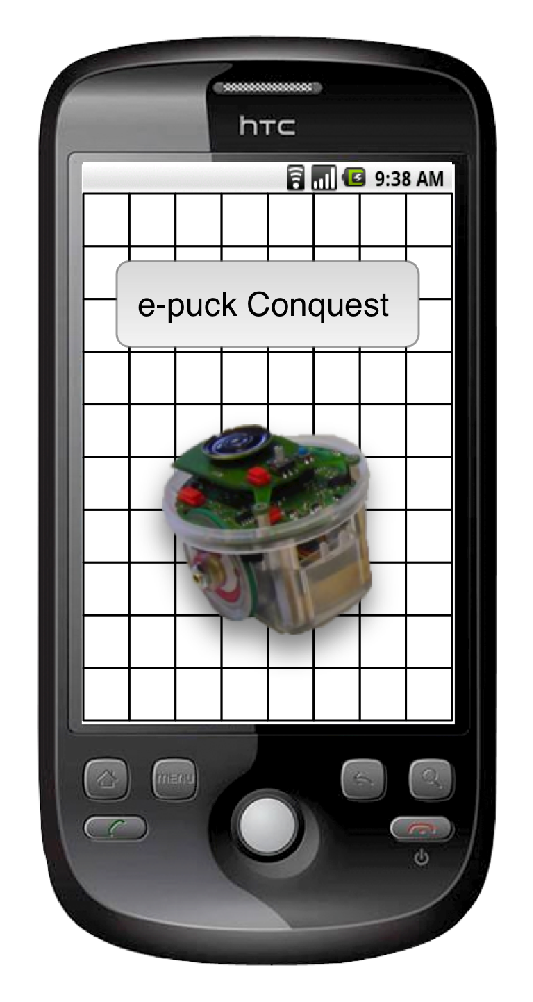
\includegraphics[height=10cm]{logo.eps} \\
%	\vspace{1cm}
	Entwurf
}
\author{
            \begin{tabular}[r]{*{3}{|c|}}
	\hline
	Phase & Verantwortlicher & E-Mail \\
	\hline \hline
	Pflichtenheft & Florian Lorenz & lorenz@fim.uni-passau.de \\
	\hline
	Entwurf & Andreas Wilhelm &  wilhelma@fim.uni-passau.de \\
	\hline
	Spezifikation & Andreas Poxrucker & poxrucke@fim.uni-passau.de \\
	\hline
	Implementierung & Martin Freund & freund@fim.uni-passau.de \\
	\hline
	Validierung & Florian Bürchner & buerchne@fim.uni-passau.de \\
	\hline
	Präsentation & Max Binder & binder@fim.uni-passau.de \\
	\hline
	\end{tabular}
}

\date{5. November 2010}

	\urldef{\astern}{\url}{http://de.wikipedia.org/wiki/A*#Funktionsweise}
	
\begin{document}

	\maketitle
	\newpage
	\tableofcontents	
	\newpage

	\section{Einleitung}
		Dieses Dokument stellt den konzeptionellen Entwurf des e-puck Conquest Systems dar. Dabei handelt es sich um ein
		verteiltes System mit bis zu sechs e-puck Roboter und einem Android-Smartphone. \\
		Die Roboter sollen ein Spielfeld möglichst zeiteffizient in Kooperation mit den anderen Teilnehmern erkunden.
		Auf dem Smartphone werden die gesammelten Kartendaten dargestellt. Außerdem kann ein e-puck zur manuellen Steuerung
		ausgewählt werden. \\ \\
		Der Entwurf des Systems wird zur besseren Übersicht in die Bereiche \textit{e-puck Roboter}, \textit{Smartphone}, \textit{abstrakte Logik}
		und \textit{Kommunikation} aufgeteilt. \\
		Das Ziel ist ein möglichst hohes Maß an Qualität, Wartbarkeit und Erweiterbarkeit. Dazu ist ein sinnvolles Systemdesign unter
		Verwendung mehrerer verschiedener Entwurfsmuster und Architekturen in allen Bereichen erforderlich. \\ \\
		Weiterhin werden in den folgenden Abschnitten die verwendeten Datentypen und Schnittstellen der Komponenten erläutert. Die beschränkten
		Ressourcen der Roboter erzwingen hierbei einen möglichst effizienten Aufbau.
		\paragraph*{Ablauf}		
		In Abbildung \ref{fig:ablauf} wird der grundsätzliche Ablauf des Systems gezeigt. Zunächst erfolgt hierbei die Kalibrierung der e-puck Roboter, um
		die Linienerkennung sinnvoll durchführen zu können. Anschließend startet der Benutzer den Erkundungsmodus des Roboters. Dabei erhält dieser
		ständig neue Fahrbefehle von den ``virtuellen e-pucks'' des Smartphones. Sobald Knoten oder Kollisionen erkannt werden, sendet der e-puck
		die entsprechenden Informationen an das Smartphone. Diese werden in den lokalen Karten der \textit{RealPucks} verarbeitet und haben
		Auswirkungen auf die folgenden Fahrbefehle.\\
		Die \textit{RealPucks} geben die Karteninformationen der realen e-pucks an das \textit{Environment} (Model) weiter, welches die globale Karte
		aufbaut und gleichzeitig für die Aktualisierung der Kartenanzeige auf dem Smartphone zuständig ist.\\
		Der Ablauf wird beendet, sobald das Spielfeld vollständig erkundet ist.		
		\begin{figure}[htbp]
			\centering
			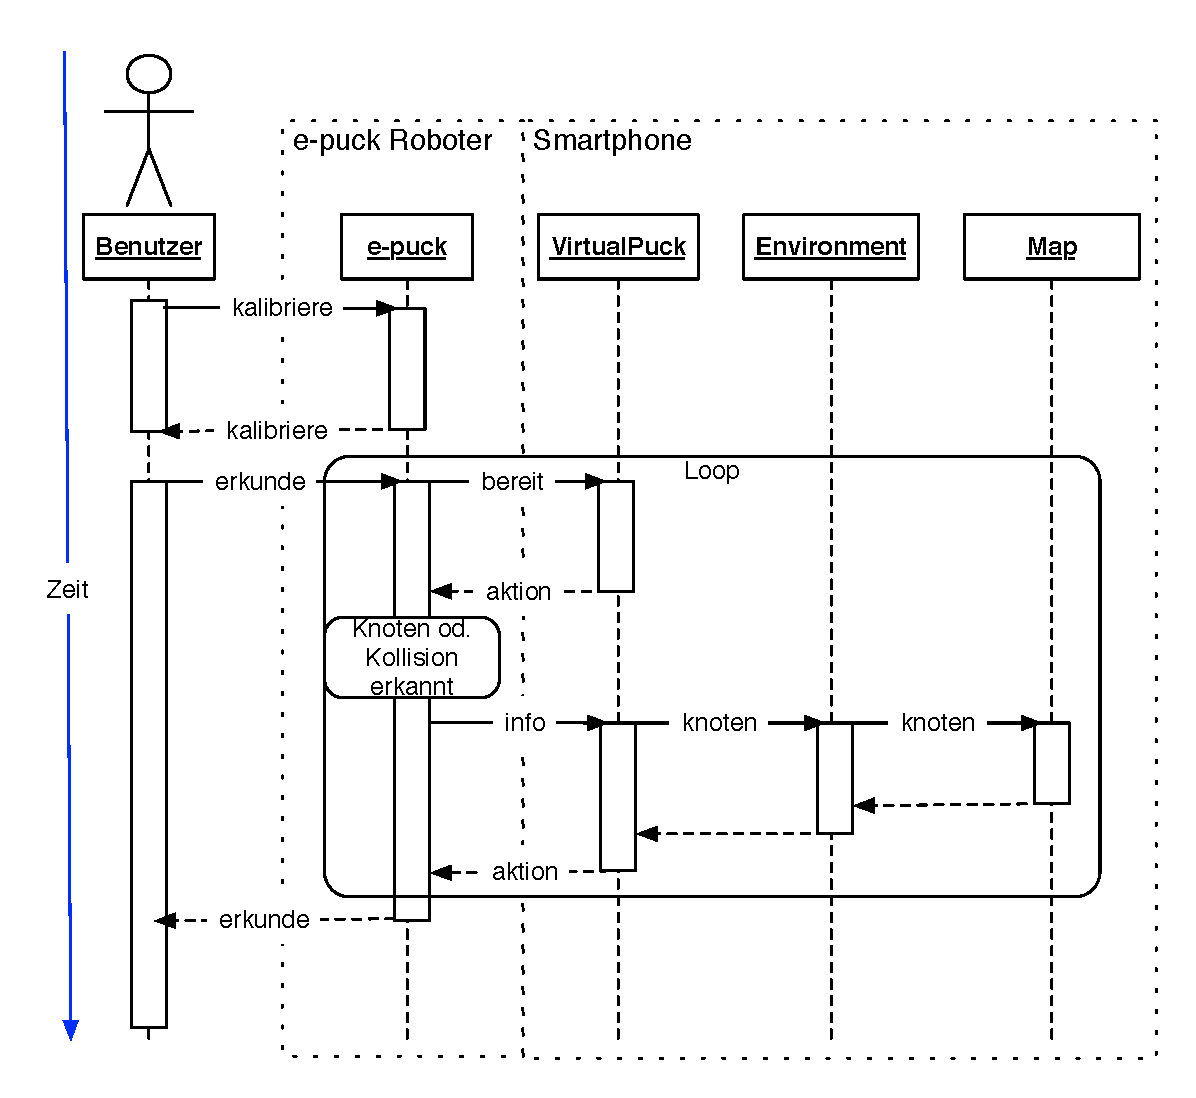
\includegraphics[width=10cm]{images/sequenzdiagramm.eps}
  			\caption{Sequenzdiagramm - Grundsätzlicher Ablauf}
  			\label{fig:ablauf}
  		\end{figure}				
	\section{e-Puck Roboter}
		Die Software des e-puck wird als Schichtenarchitektur mit wachsendem Abstraktionsgrad entworfen. \\
		Jede Schicht besteht aus einer oder mehreren Komponenten. Diese sind teilweise wiederum aus mehreren
		Schichten aufgebaut. \\
		
		\begin{figure}[h]
			\centering
			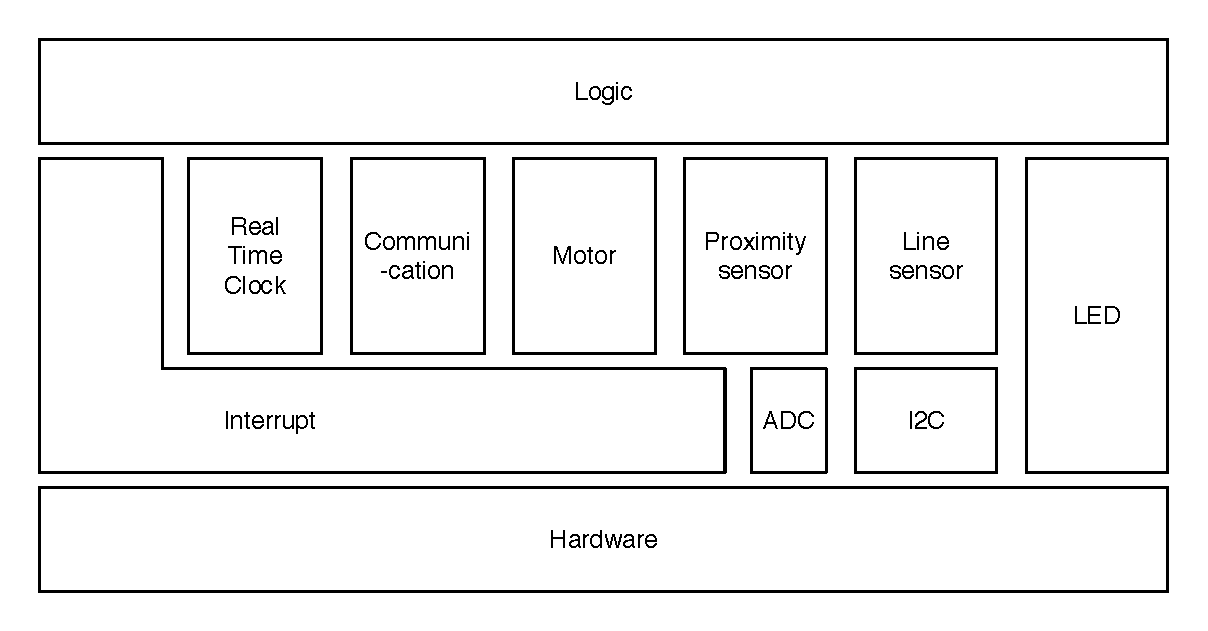
\includegraphics[width=10cm]{images/e-puck_architecture.eps}
  			\caption{Architektur der Software des e-puck}
  		\end{figure}
		
		Die folgenden Abschnitte beschreiben die einzelnen Komponenten der Architektur näher.
		 
			\paragraph*{Komponente `Interrupt'}
			Die Komponente `Interrupt' bietet einfache Funktionen zum globalen Ein- und Ausschalten von Interrupts und zur Festlegung
			von Interrupt-Prioritäten. Außerdem können gesetzte Interrupt-Flags gelöscht werden. \\ \\
			Diese Funktionen werden in den Komponenten `Timer', `Motor', `Communication' und `IR proximity sensor' sowie
			in der darüber liegenden Logikschicht verwendet. \\
			
			Strukturelle Gliederung der Komponente:
			\begin{verbatim}  
			hal_int.h, hal_int.c, hal_int_types.h
			\end{verbatim}

			\paragraph*{Komponente `Real-Time-Clock'}
			Die `Real-Time-Clock'-Komponente stellt eine Echtzeituhr bereit. Diese speichert die aktuelle Laufzeit des e-puck Roboter und löst in
			regelmäßigen Abständen Interrupts aus.
			Außerdem können Callbacks für zeitgesteuerte Funktionen anderer Komponenten registriert werden. \\
			
			Strukturelle Gliederung:
			\begin{verbatim}  
			hal_rtc.h, hal_rtc.c, hal_rtc_types.h
			\end{verbatim}
			
			\paragraph*{Komponente `Communication'}
			Die Komponente `Communication' stellt einfache Funktionen zum Aufbau und zur Verwaltung  der Bluetooth-Verbindung bereit.
			Sie enthält außerdem Funktionen zum Senden und Empfangen von Bluetooth-Nachrichten.\\
			 
			Dieses Modul besteht aus zwei aufeinander aufbauenden Komponenten mit wachsendem Abstraktionsgrad:
			
				\subparagraph*{hal\_uart1}
				Diese Komponente enthält Funktionen zur Initialisierung des UART. Insbesondere werden das Datenformat und die Datenrate festgelegt.
				Darüber hinaus können die Sende- und Empfangs-Interrupts des UART konfiguriert werden. Die zu den Interrupts gehörigen Interrupt
				Service Routinen sind ebenfalls Teil der Komponente. \\
				Auch die Kontrolle des Transmitter (Tx)- und Receiver (Rx)-Ringpuffers wird in diesem Modul realisiert. \\
				Das Senden und Empfangen von Nachrichten erfolgt asynchron. \\
				
				Strukturelle Gliederung:
				\begin{verbatim}  
				hal_uart1.h, hal_uart1.c, hal_uart_types.h
				\end{verbatim}
				
				Externe Datenstrukturen: \\
				ringbuf\_SContext\_t: Zustand des Ringpuffers
				
				\lstset{language = C, tabsize = 4}
				\begin{lstlisting}[captionpos=b, caption={ringbuf\_SContext\_t}, frame = single]
typedef struct {
	uint8_t* lpui8Storage;
	uint16_t ui16Size;
	volatile uint16_t ui16ReadIndex;
	volatile uint16_t ui16WriteOffset;
} ringbuf_SContext_t;
				\end{lstlisting}
				
				\subparagraph*{com}
				`com' enthält Funktionen zur Generierung von Raw-Messages (Nachrichten, die vom Bluetooth-Modul versendet werden
				können) und zur Aufbereitung von eingehenden Raw-Nachrichten aus der darunter liegenden `hal\_uart1'-Schicht. \\
				
				Strukturelle Gliederung:
				\begin{verbatim}  
				btm.h, btm.c, btm_types.h
				\end{verbatim}
				
				Externe Datenstrukturen: \\
				com\_SMessage\_t: Format der Raw-Nachrichten
				
				\lstset{language = C, tabsize = 4}
				\begin{lstlisting}[captionpos=b, caption={com\_SMessage\_t}, frame = single]
typedef struct {
	uint16_t ui16type;
	uint8_t aui8Data[30];
} com_SMessage_t;
				\end{lstlisting}
				
			\paragraph*{Komponente `Motor'}
			Das Modul `Motor' stellt Funktionen zur Verfügung, die die Voraussetzung für die High-Level-Steuerung der Bewegung des e-puck bilden.
			Die Komponente initialisiert und kontrolliert die Timer für die Steuerung der beiden Schrittmotoren und gewährleistet deren korrekte
			Ansteuerung. \\
			Außerdem werden Funktionen bereit gestellt, mit denen die Geschwindigkeit der beiden Motoren eingestellt werden kann und deren
			Schrittzähler gelesen und gesetzt werden können. \\
			
			Strukturelle Gliederung:
				\begin{verbatim}  
				hal_motor.h, hal_motor.c, hal_motor_types.h
				\end{verbatim}
						
			\paragraph*{Komponente `ADC'}
			Die Komponente `ADC' kapselt Funktionen zur Initialisierung der Analog-Digital-Wandler und zum einfachen Auslesen der Register
			mit den konvertierten Werten. \\
			Die Funktionen der Komponente bilden eine wichtige Grundlage für die Verwendung der IR-Abstandssensoren und werden vom Modul `IR 
			proximity sensor' verwendet.\\
			
			Strukturelle Gliederung:
				\begin{verbatim}  
				hal_adc.h, hal_adc.c, hal_adc_types.h
				\end{verbatim}
			
			\paragraph*{Komponente `I2C'}
			Die Komponente `I2C' initialisiert die Datenrate und die Masterfunktionalität des I2C-Moduls.
			Außerdem werden grundlegende Übertragungsfunktionen wie Adressierung, Lesen und Schreiben zur Verfügung gestellt. \\
			
			Strukturelle Gliederung:
				\begin{verbatim}  
				hal_i2c.h, hal_i2c.c
				\end{verbatim}
			
			\paragraph*{Komponente `IR proximity sensor'}
			Diese Komponente erfüllt im wesentlichen zwei Aufgaben.
			Zunächst findet eine Initialisierung statt. Hierbei wird das Abtastintervall mit dem die Sensoren ausgelesen werden definiert und der 
			Timer eingerichtet, mit dem das Abtastintervall betrieben wird.
			Weiterhin stellt dieses Modul die Funktionen zum Auslesen der IR-Sensoren zur Verfügung. Dabei werden Funktionen der `ADC'-Komponente 		
			verwendet. \\
			
			Strukturelle Gliederung:
				\begin{verbatim}  
				sen_prox.h, sen_prox.c, sen_prox_types.h
				\end{verbatim}
			
			\paragraph*{Komponente `Line sensor'}
			Die Hauptaufgabe dieser Komponente liegt darin, die Daten der IR-Abstandssensoren aus dem I2C-Bus auszulesen. Diese Daten werden 
			einem Regler zur Verfügung gestellt, der gewährleistet, dass der Roboter seine Linie nicht verlässt. \\
			
			Strukturelle Gliederung:
				\begin{verbatim}  
				sen_line.h, sen_line.c, sen_line_types.h
				\end{verbatim}

			\subparagraph*{Sensordaten}
				Die Linien- und Knotenerkennung erfolgt über die drei Bodensensoren. Wie in Abbildung \ref{fig:auswertung} zu sehen ist,
				können dunkle Abschnitte besonders gut erkannt werden. Eine sinnvolle Linien- und Knotenerkennung kann bereits bei einem Schwarzwert von
				70 Prozent durchgeführt werden.
				\begin{figure}[h]
					\centering
					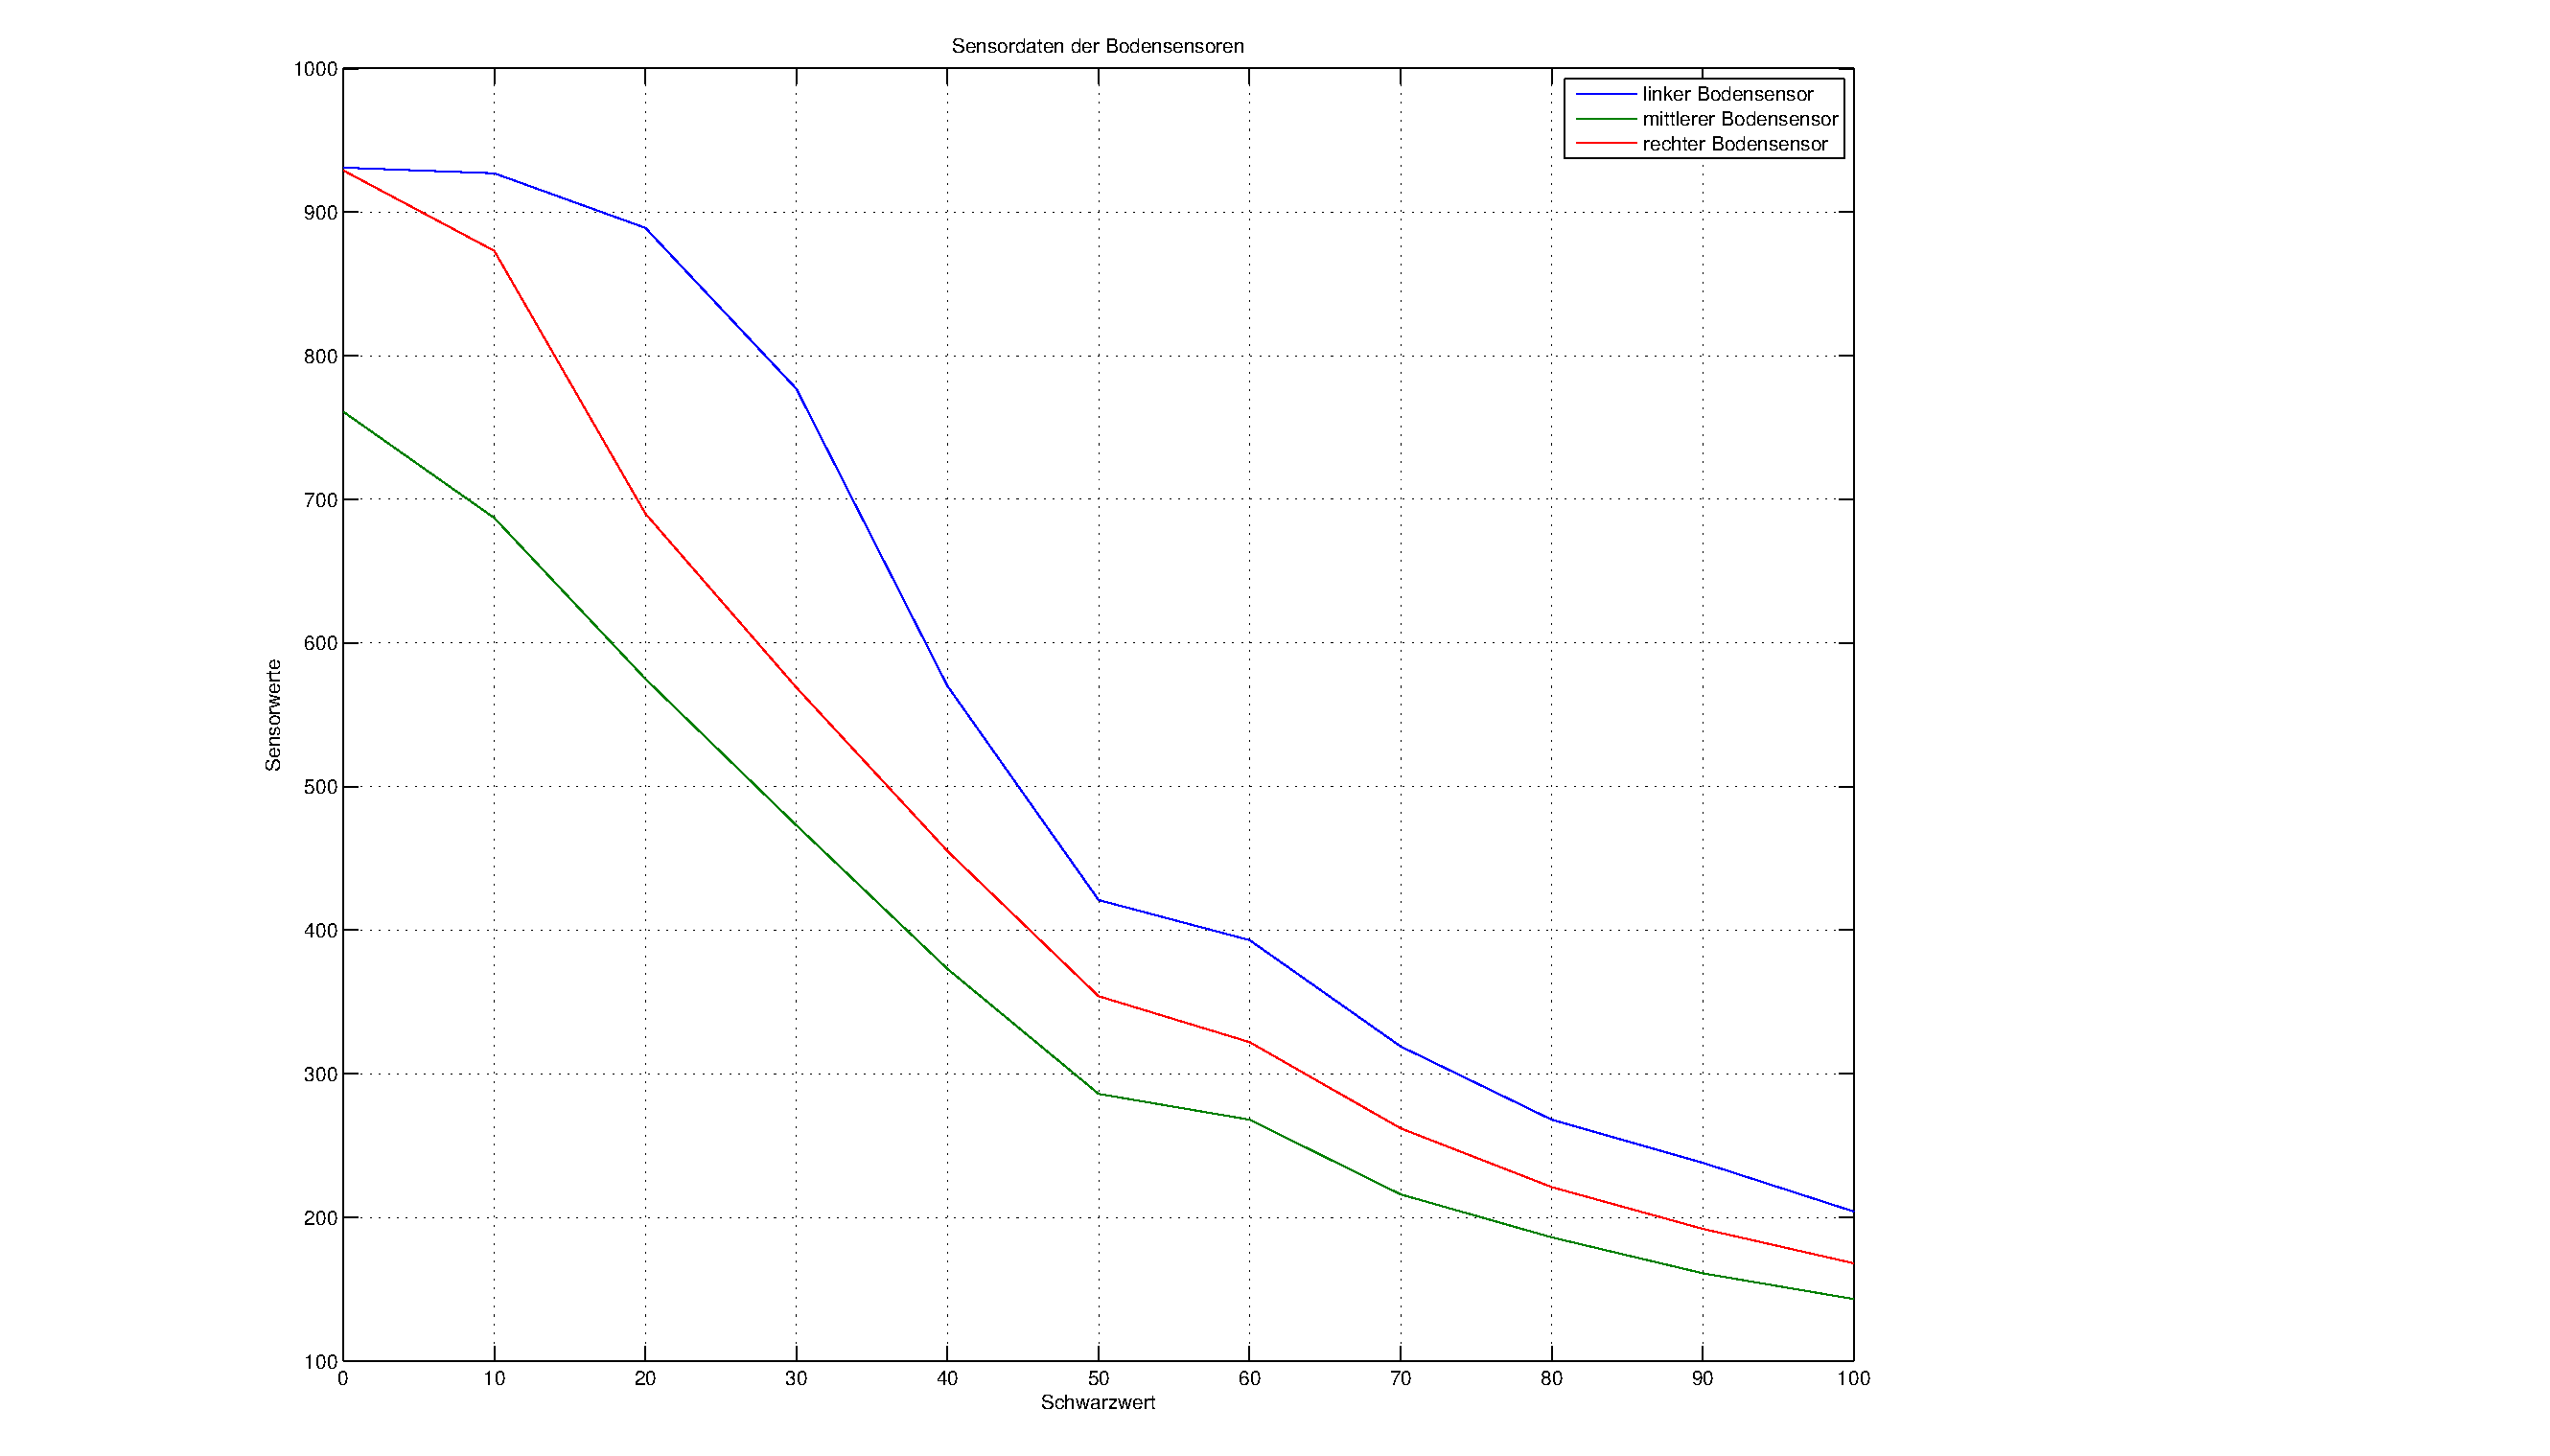
\includegraphics[width=18cm]{images/sensorgrafik.eps}
					\caption{Verhalten der Sensoren}		
					\label{fig:auswertung}	
				\end{figure}
			
			\paragraph*{Komponente `LED'}
			Zunächst werden sämtliche für die LEDs benötigten Hardware-Register initialisiert. Sobald dies geschehen ist, kann durch diese Komponente
			die Ansteuerung der LEDs am e-puck übernommen werden.
			
			Strukturelle Gliederung:
				\begin{verbatim}  
				hal_led.h, hal_led.c
				\end{verbatim}

		\paragraph*{Komponente `Logic'}
			Diese Komponente des Systems basiert auf allen zuvor genannten Komponenten und wird in einer Subsumption-Architektur umgesetzt. Hierbei
			handelt es sich um ein nach Prioritäten geordnetes Schichtenmodell, welches in jedem Roboter in den Dateien \texttt{subs.c} und 
			\texttt{subs.h} enthalten ist. Jede Schicht definiert einen Verhaltensaspekt des jeweiligen e-pucks und besitzt Zugriff auf globale Variablen,
			welche Sensordaten speichern. \\
            In Abbildung \ref{fig:subsumption} wird die Anordnung der Schichten nach Priorität veranschaulicht. \\ 

			\begin{figure}[h]
				\centering
				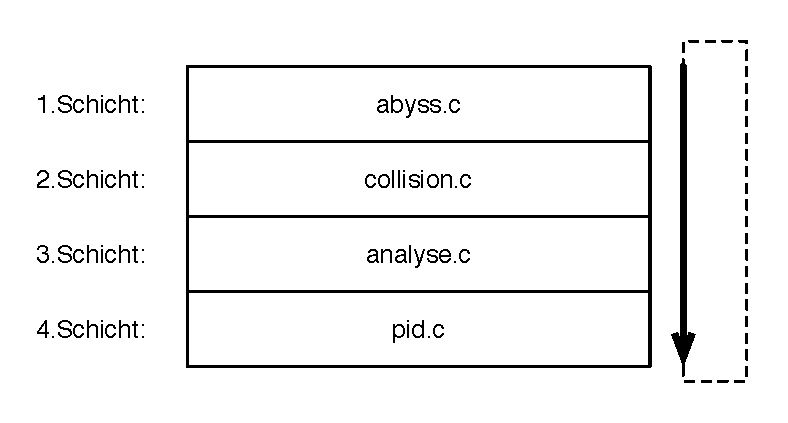
\includegraphics[height=5cm]{images/subsumption.eps}
				\caption{Subsumption-Stack}		
				\label{fig:subsumption}	
			\end{figure}

			Niedrige Schichten beschreiben also die grundlegendsten und wichtigsten Verhaltensweisen eines e-pucks, während höhere Schichten zunehmend
			abstrakteres Verhalten beschreiben und nur dann ausgeführt werden, wenn nicht bereits ein wichtigeres Verhalten ausgeführt wurde. Weitere,
			komplexere Verhaltensschichten können dadurch problemlos ergänzt werden.\\ 
			In diesem System wird jeder e-puck einen Verhaltenskodex gemäß obiger Abbildung befolgen. \\
			Je nach Sensordaten kommt ein bestimmtes Verhalten zur Ausführung, wobei höher liegende Verhaltensschichten ignoriert werden bis das
			angestrebte Ziel erreicht wurde bzw. kritische Daten vom Sensor gemeldet wurden. Anschließend wird eine Liste der registrierten Verhalten
			erneut von vorne durchlaufen. \\
			Die einzelnen Verhaltensschichten befinden sich gekapselt in einzelnen C-Dateien, so dass sie einfach und schnell ausgetauscht, erweitert und
			gewartet werden können. Diese Schichten werden im Folgenden näher erläutert. \\

			\begin{enumerate}
  				\item Schicht 0: Kalibrierung \\
					Damit die Unterscheidung von Linien zum Untergrund optimal durchgeführt werden kann, ist eine Kalibrierung notwendig. Diese kann
					zwar auf dem EEPROM des e-pucks persistent gespeichert werden, muss allerdings bei wechselnden Lichtverhältnissen oder Untergrund
					erneut durchgeführt werden. \\
					Für die Kalibrierung muss der Benutzer den Selektor am Roboter auf Position 0 stellen und ihn auf eine Linie des entsprechenden
					Spielfelds stellen. Im Abstand von 5 Zentimetern vor der Linie in Fahrtrichtung darf hierbei keine Linie sein, sondern die
					Hintergrundfläche, die später beim Betrieb verwendet wird. Nach dem Einschalten des e-pucks speichert dieser zunächst die Werte der
					Bodensensoren auf der Linie, fährt anschließend um 250 Motorschritte (ca. eine viertel Umdrehung) vorwärts und speichert erneut
					die Werte auf der Hintergrundfläche. Der Roboter ist nun fertig kalibriert und bereit für den Start des Systems, wobei die Position des
					Selektors auf eine Position ungleich 0 gestellt wird.

					\begin{verbatim} 
					subs_calibrate.c, subs_calibrate.h
					\end{verbatim}			
			
  				\item Schicht 1: Abgrund \\
					Diese Schicht wird aktiv sobald die Bodensensoren einen Abgrund erkennen. Diese kritische Situation muss mit oberster 
					Priorität behandelt werden indem die Motoren sofort gestoppt werden und eine Meldung an das Smartphone erfolgt.

					\begin{verbatim} 
					subs_abyss.c, subs_abyss.h
					\end{verbatim}

  				\item Schicht 2: Kollision \\
					Diese Schicht der Subsumption-Architektur wird ausgeführt sobald einer der acht IR-Sensoren, die rundherum außen am Roboter 
					angebracht sind einen kritischen Wert liefert. Dann nämlich wurde erkannt, dass eine Kollision unmittelbar bevorsteht. Daraufhin wird
					eine Kollisionsmeldung an das Smartphone gesendet.

					\begin{verbatim}  
					subs_collision.c, subs_collision.h
					\end{verbatim}

				\item Schicht 3: Knotenanalyse \\
					Hier werden die Daten der Bodensensoren verarbeitet um zu entscheiden ob der Roboter soeben einen Knoten passiert hat und welche
					Beschaffenheit dieser besitzt. Falls ein Knoten ermittelt werden konnte wird dessen Art an dass Smartphone gemeldet und auf
					die nächste Anweisung gewartet.	\\
					Die Knotenanalyse erkennt einen Knoten, sobald der linke oder rechte Bodensensor bei mehr als drei Motorschritten einen besonders
					deutlichen Schwarzwert feststellt. Wie in Abbildung \ref{fig:auswertung} zu sehen, werden Sensorwerte bereits bei 70 Prozent des
					Weiß-Wertes gute Unterscheidungen erreicht. Um auch bei ungünstigen Lichtverhältnissen eine gute Erkennung zu ermöglichen,
					werden Knoten ab einem Sensorwert von 50 Prozent des Weiß-Wertes festgestellt. Um keine störenden Kurven bei Knoten mit nur einem
					Ast zu fahren, wird die Linienverfolgung für die Zeit des Knotens deaktiviert. 				

					\begin{verbatim}  
					subs_analyse.c, subs_analyse.h
					\end{verbatim}

				\item Schicht 4: Bewegungsmodifikationen \\
					Die Aufgabe dieses Teils der Verhaltensarchitektur ist es die Befehle des Handys (vom zugehörigen \textit{RealPuck}) bezüglich
					Geschwindigkeitsänderungen und Drehungen	 umzusetzen. Dies kann nur unmittelbar nach einer erfolgreichen Knotenanalyse
					inklusive Rückmeldung des Smartphones geschehen. Der e-puck befindet sich zu diesem Zeitpunkt auf einem Knoten.			

					\begin{verbatim}  
					subs_move.c, subs_move.h
					\end{verbatim}

  				\item Schicht 5: Linienverfolgung \\
					Diese Schicht verwendet die Daten der Bodensensoren, um mit Hilfe eines PID-Reglers dafür zu sorgen, dass der e-puck die Linie
					nicht verlässt. \\

					\begin{verbatim}
					subs_pid.c, subs_pid.h
					\end{verbatim}

  			\end{enumerate}

		\section{Smartphone}
			In Abbildung \ref{fig:klassendiagramm} wird das Klassendiagramm der Android-Anwendung dargestellt. Die einzelnen Klassen und Abläufe
			sind in den folgenden Kapiteln näher erläutert. Dazu werden auch Teile des Diagramms zur Veranschaulichung verwendet. \\
			\begin{figure}[p]
				\centering
				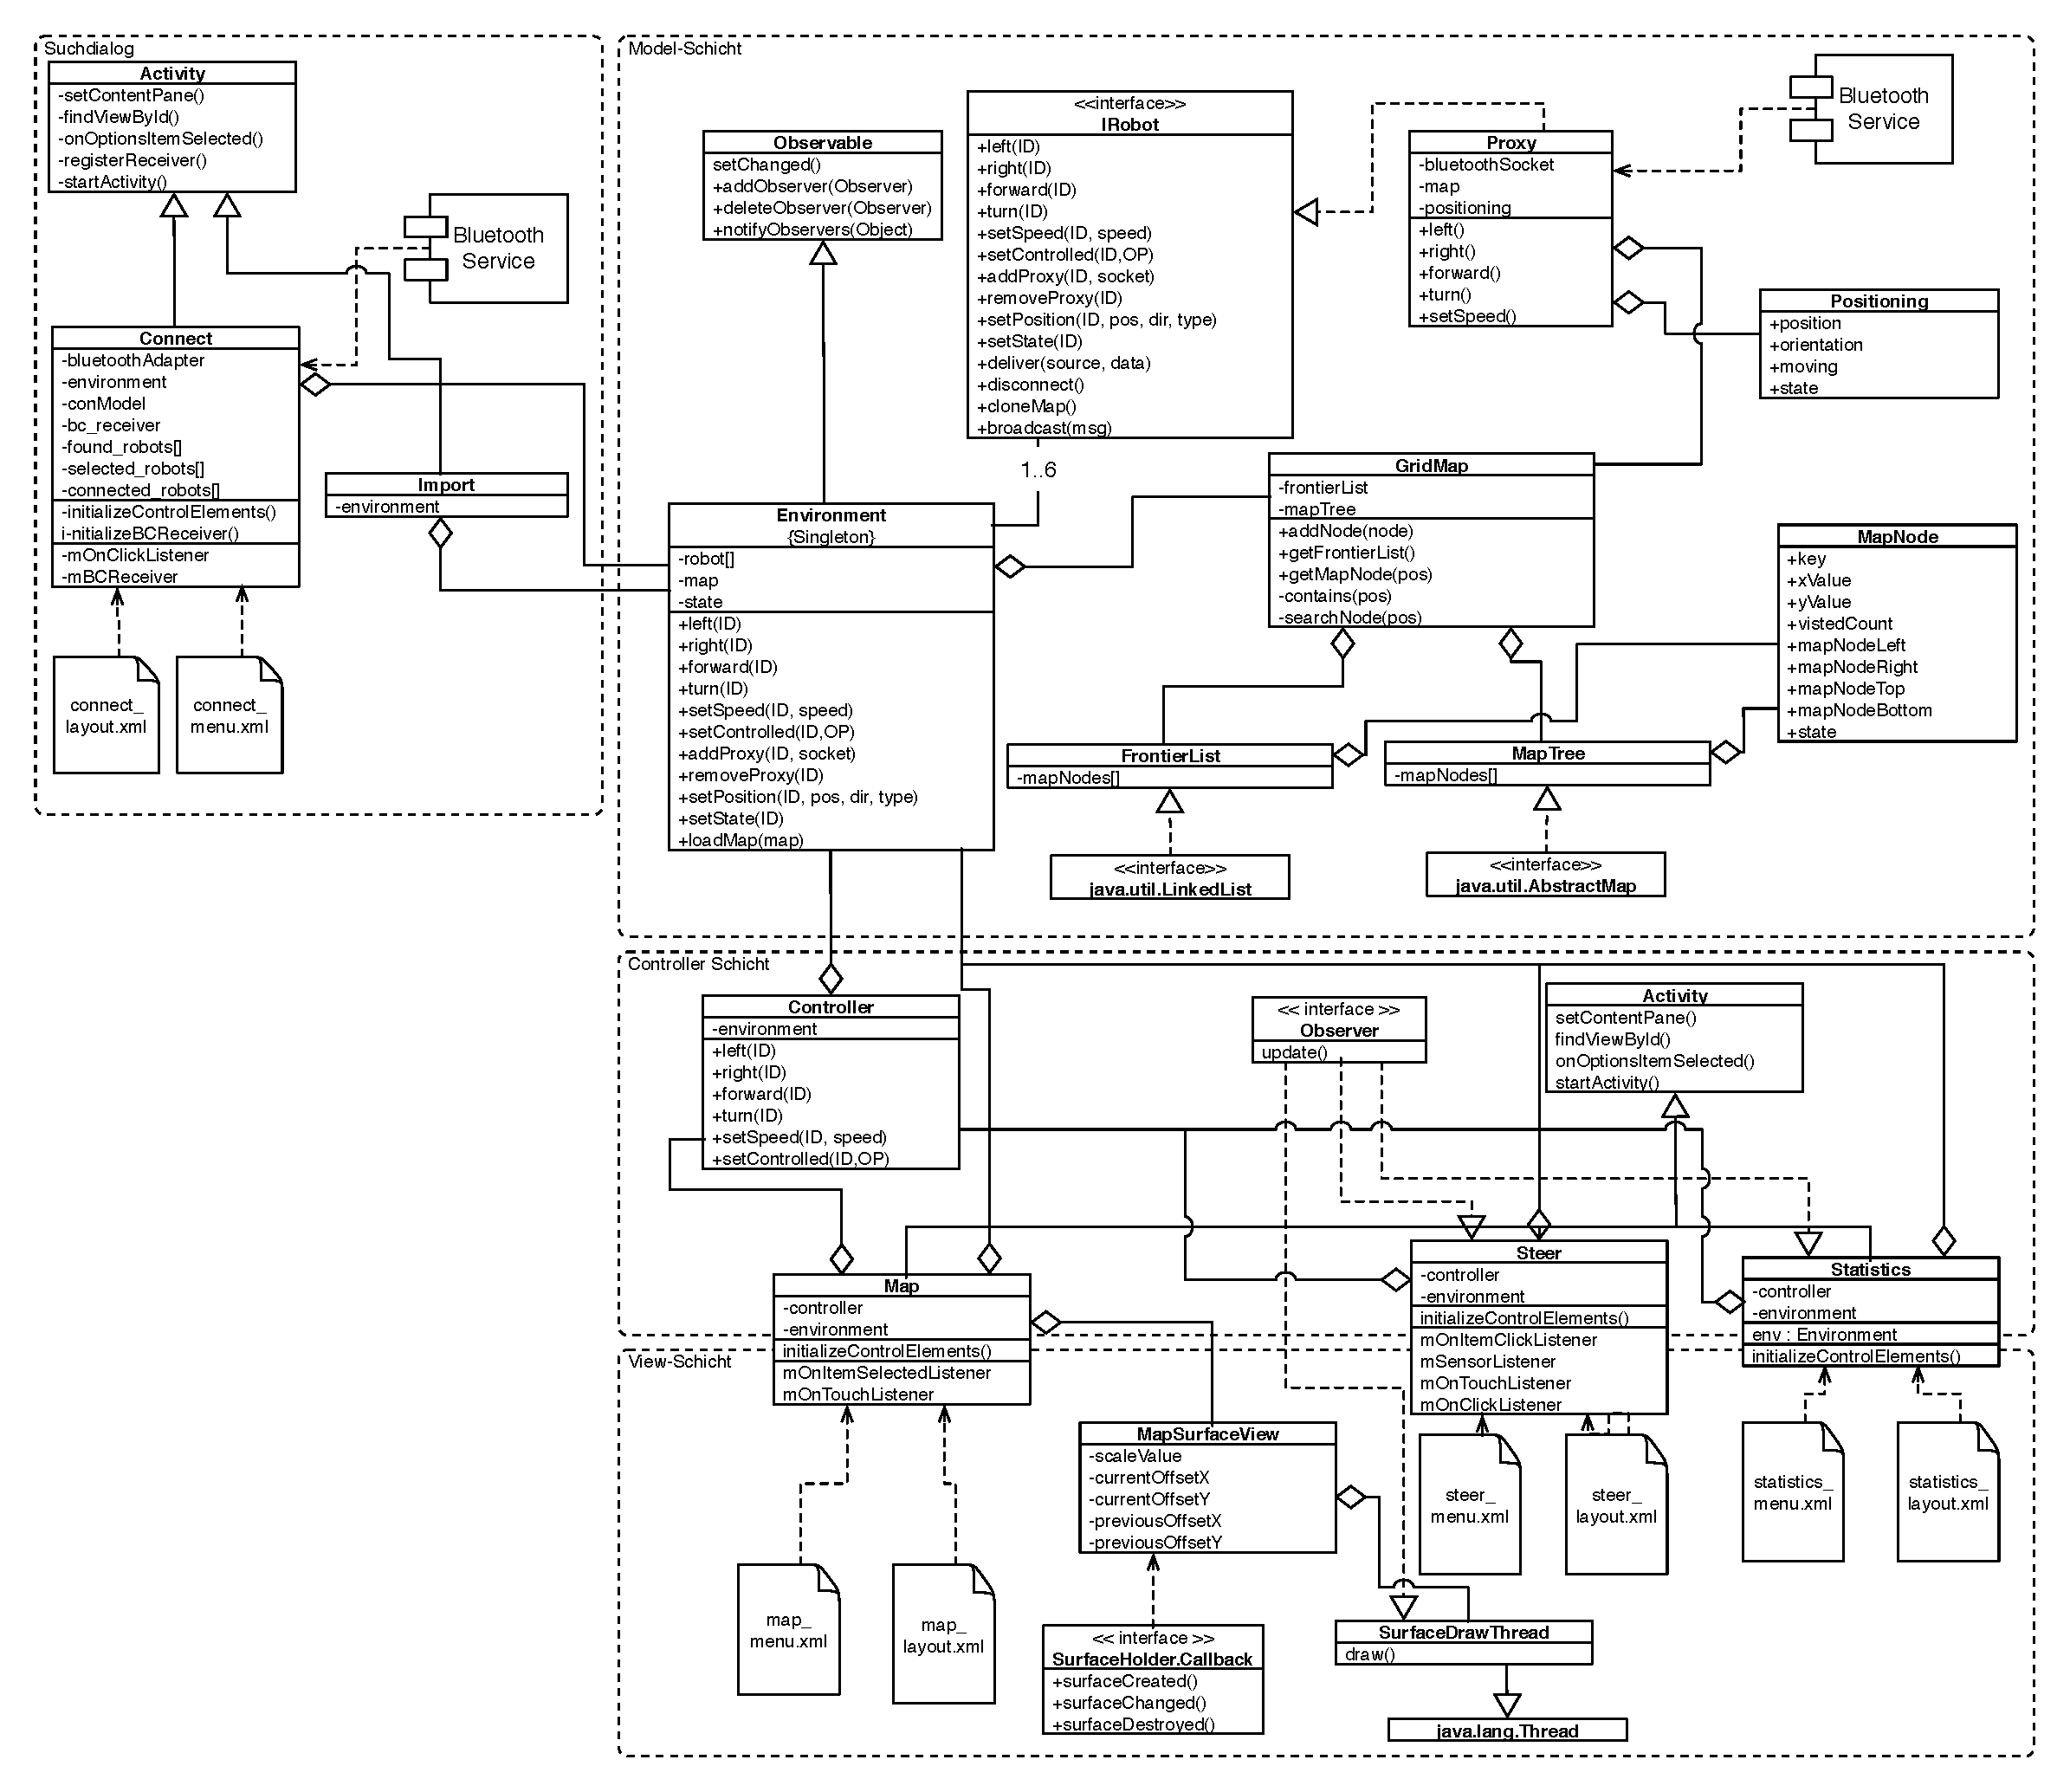
\includegraphics[width=18cm, angle=90]{images/android_klassendiagramm.eps}
  				\caption{Klassendiagramm - Android Anwendung}
  				\label{fig:klassendiagramm}
  			\end{figure}	

			\subsection{Beschreibung der verwendeten Klassen}
			\paragraph*{\textbf{Connect}} erbt von der Klasse \textit{Activity} und ermöglicht die Suche nach verfügbaren e-puck Robotern. Diese werden
			aufgelistet angezeigt Außerdem stellt die Activity die Verbindung zu den ausgewählten e-pucks her.
			\paragraph*{\textbf{Import}} erbt von der Klasse \textit{Activity} und ermöglicht das Auswählen und Öffnen einer abgespeicherten Karte.
			\paragraph*{\textbf{Simulation}} erbt von der Klasse \textit{Activity} und ermöglicht die Ausführung der Anwendung im Simulationsmodus.
			Es kann die zu simulierende Karte und die Anzahl der teilnehmenden e-puck Roboter eingestellt werden.
			\paragraph*{\textbf{CommunicationManager}} implementiert das Interface \textit{IComMan} und regelt die Kommunikation zwischen den Instanzen der
			\textit{Puck}-Klassen einerseits und Instanzen der \textit{Puck}-Klassen mit dem \textit{Environment} andererseits.
			\paragraph*{\textbf{Environment}} erbt von der Klasse \textit{Observable}. Sie bildet das Model der MVC-Architektur.
			\paragraph*{\textbf{Puck}} ist die abstrakte Oberklasse der Klassen \textit{VirtualPuck} und \textit{RealPuck}. Sie enthält die lokale Karte
			sowie Informationen zur eigenen Position und die Position der anderen Roboter. Außerdem ist die Verhaltenslogik der Roboter in Form eines Threads
			realisiert.
			\paragraph*{\textbf{VirtualPuck}} erbt von der abstrakten Klasse \textit{Puck} und stellt einen virtuellen e-puck für den Simulationsmodus dar.
			Die für die Erkundung notwendigen Informationen (z.B. Knotentypen) erhält der \textit{VirtualPuck} durch den \textit{Simulator}.
			\paragraph*{\textbf{RealPuck}} erbt von der abstrakten Klasse \textit{Puck} und stellt einen realen e-puck für den normalen Erkundungsmodus
			dar. Die für die Erkundung notwendigen Informationen tauscht der \textit{RealPuck} durch Bluetooth-Kommunikation mit dem realen e-puck Roboter
			aus.
			\paragraph*{\textbf{Simulator}} stellt den \textit{VirtualPuck}s im Simulationsmodus alle relevanten Informationen (z.B. Startpositionen und
			Knotentypen) zur Verfügung.
			\paragraph*{\textbf{Positioning}} ist eine Containerklasse, die den aktuellen Zustand des \textit{Puck}s sowie dessen aktuelle Position
			speichert.
			\paragraph*{\textbf{GridMap}} wird als Struktur zur Speicherung der Karte verwendet.
			\paragraph*{\textbf{MapNode}s} sind die Bausteine der \textit{GridMap}. Sie speichern u.a. Koordinaten, Referenzen auf Nachbarknoten und die Art
			des Knotens.
			\paragraph*{\textbf{AStarNode}} ist eine Erweiterung der Klasse \textit{MapNode} und wird für den A*-Algorithmus verwendet.
			\paragraph*{\textbf{LogicThread}} ist für die Ausführung der zustandsabhängigen Verhaltenslogik und zuständig und steuert die Kommunikation des
			zugehörigen \textit{Puck}s.
			\paragraph*{\textbf{ConcreteBehaviour}-Klassen} implementieren das Interface \textit{IBehaviour} und enthalten die zustandsabhängige
			Verhaltenslogik der \textit{Puck}s.
			\paragraph*{\textbf{AStarPathFinder}} implementiert das Interface \textit{IPathFinder} und enthält den A*-Algorithmus.
			\paragraph*{\textbf{Handler}} ist eine abstrakte Klasse, die als Oberklasse für konkrete \textit{Handler}-Klassen zur Behandlung von eingehenden
			Nachrichten verwendet wird.
			\paragraph*{\textbf{ConcreteHandler}} erben von der abstrakten \textit{Handler}-Klasse und implementieren die konkrete Behandlung je eines
			speziellen Nachrichtentyps.
			\paragraph*{Controller}
			überwacht alle Views auf Eingaben durch den Benutzers, verarbeitet diese und reicht sie an das Environment weiter.
			\paragraph*{Steer}
			erbt von Activity und bietet Funktionen zur Auswahl, sowie zwei Arten zur Steuerung der Roboter an.
			\paragraph*{Statistics}
			erbt ebenfalls von Activity. Hier wird der Erkundungsvorgang aller Roboter in einer Statistik aufbereitet und dargestellt.
			\paragraph*{Map}
			erbt von Activity und stellt die Auswahl aller angemeldeten Roboter zur Verfügung. Außerdem beinhaltet sie die MapSurfaceView.
			\paragraph*{MapSurfaceView}
			erbt von der Klasse SurfaceView und implementiert die Interfaces SurfaceHolder.Callback und View.OnTouchListener.
			Sie ist eine innere Klasse von Map und dient der Visualisierung der bereits erkundeten Fläche durch die Roboter.
			\paragraph*{SurfaceDrawThread}
			ist eine innere Klasse der MapSurfaceView. Sie erbt von der Klasse Thread und implementiert das Interface Observer. 
			Sie reagiert auf Änderungen in der Datenstruktur der Karte und stellt diese grafisch dar.
			\subsection{Beschreibung der verwendeten Interfaces}
			\paragraph*{IComMan}
			Klassen die dieses Interface implementieren sind dadurch in der Lage den Broadcast von Nachrichten durchzuführen.
			\paragraph*{IRobot}
			Dieses Interface sichert die Möglichkeit der Anbindung unterschiedlicher Robotertypen an den Communication Manager.
			\paragraph*{IPathFinder}
			Das Interface IPathFinder dient zur Implementierung von Klassen, welche Knoten finden und die Kosten zwischen diesen berechnen müssen. 
			\paragraph*{IBehaviour}
			Dieses Interface regelt das Verhalten der Roboter im Bezug auf Kollisionsvermeidung und Wegfindung.


			\subsection{Model-View-Controller (MVC) Architektur}
				Die Daten- bzw. Benutzer-Interaktion der Android-Anwendung wird mit einer MVC-Architektur aufgebaut. Dies ermöglicht ein
				flexibles Programmdesign, das eine Wiederverwendbarkeit von Komponenten sowie eine reduzierte Komplexität gewährleistet.
				Die Daten, wie z.B. Karteninformationen oder Roboterpositionen, können dadurch von den zugehörigen Darstellungen getrennt werden
				(\textit{Separation of Concerns}). Es werden hierbei drei Dialoge (\textit{Activities}) verwendet, je ein Dialog für Kartenansicht, Steuerung und
				Statistik. Bei diesem Entwurf hat die View-Schicht keinen direkten Zugriff auf das Model, dieser wird vollständg vom
				Controller übernommen. Gemäß den Entwicklerrichtlinien für Android-Anwendungen 
				\footnote{Android-User Interface (\url{http://developer.android.com/guide/topics/ui/index.html})} gehören die Activity-Klassen der
				View logisch zum	Controller. Die Model-Schicht (\textit{RealPuck}) erhält über die Bluetooth-Schnittstelle Aktualisierungen der e-puck Roboter,
				welche den Zustand ändern.\\
				Die beschriebenen Steuerungs- und Dialogabläufe werden hier nur rudimentär zum Verständnis erwähnt. Eine genauere Erläuterung ist in
				Kapitel \ref{sec:aufbau_dialoge} zu finden
	  			\begin{figure}
					\centering
					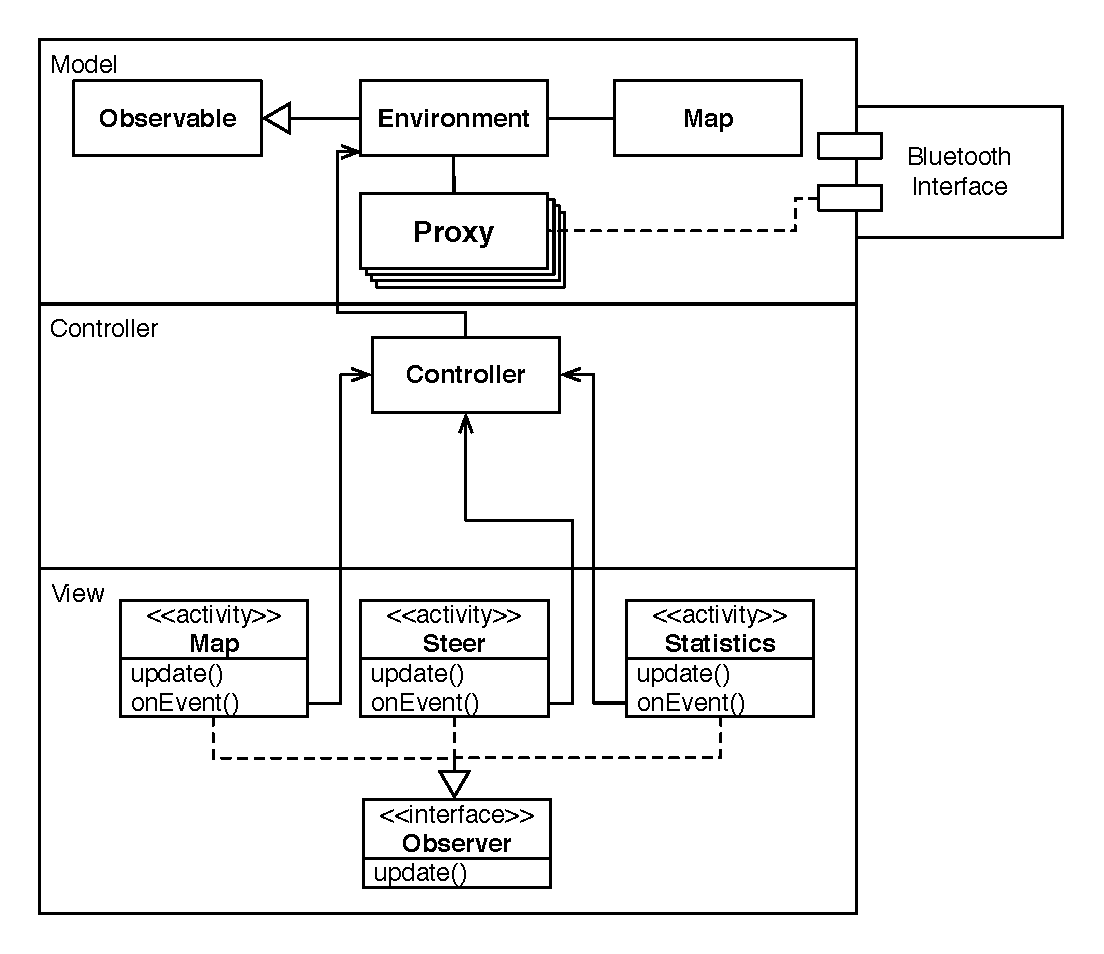
\includegraphics[width=10cm]{images/android_mvc.eps}
  					\caption{Model-View Controller Architektur}
  					\label{fig:mvc}
 	 			\end{figure}					
			\paragraph*{Model}
  				Die Model-Schicht der Architektur speichert als zentrale Komponente sämtliche Daten bzgl. Karten- und e-puck-Informationen. 
  				Sie beinhaltet außerdem die Applikationslogik der Android-Anwendung. Die Kommunikation nach außen findet im Erkundungsmodus
  				mit realen e-pucks über die Bluetooth-API statt. Die Klasse \textit{Environment} erbt von der Klasse \textit{Observable} und verarbeitet
  				die Aktualisierungen der Roboter. Die Klasse wird als Singleton realisiert, da hier globale Zustandsdaten und Karteninformation
  				für die Anzeige gespeichert werden. Informationen der einzelnen Roboter, sowie deren Ablaufsteuerung, werden in den Instanzen
  				der Klasse \textit{RealPuck} verwaltet (siehe Kapitel \ref{sec:repraesentation}). Diese Instanzen werden in einer Attributsliste der Klasse
  				\textit{CommunicationManager} gehalten und besitzen auch selbst einen Verweis auf den Kommunikations-Manager. Bei Zustandsänderung
  				der \textit{RealPuck}-Instanzen bzw. bei Änderung der Kartendaten werden die registrierten Views benachrichtigt.
  			\paragraph*{View}
  				Die Präsentationskomponenten der MVC-Architektur sind für die Ausgabe der Model-Daten zuständig und bilden eine
  				Abstraktionsschicht zwischen der Präsentation der Anwendung, dem Model und dem Benutzer. Die Schicht besteht aus den drei
  				Klassen	\textit{Map}, \textit{Steer} und \textit{Statistics}. \textit{Map} ist für die Kartendarstellung
  				verantwortlich, \textit{Steer} stellt die Steuerungsbedienelemente dar und \textit{Statistics} beinhaltet statistische
  				Informationen.  Damit die View-Klassen als \textit{Activities} für die Android-Applikation verwendet werden können, müssen sie
  				von der Klasse \textit{Activity} erben. Für die Verwendung als View der MVC-Architektur muss zusätzlich das Interface
  				\textit{Observer} implementiert werden\footnote{Die Activity \textit{Map} stellt eine Ausnahme dar, da hier ein \textit{Surface View} als
  				Darstellung verwendet wird. Die Aktualisierung geschieht hierbei über einen extra Thread. Daher muss dieser auch als Observer eingetragen
  				werden (siehe Abschnitt \ref{subsec:dialog_map})}. Jede einzelne View registriert sich bei der Klasse \textit{Environment} als Observer,
  				um bei Zustandsänderungen vom Model benachrichtigt zu werden. Benutzereingaben auf den Dialogen werden über
  				die Ereignisbehandler-Methoden der \textit{Activity}-Klasse an das Model weitergegeben. Somit gehören diese Handler-Methoden
  				im Sinne der MVC-Architektur der Controller-Schicht an.
  			\paragraph*{Controller}
  				Der Controller nimmt Eingaben aus den verschiedenen View Klassen entgegen und leitet diese bereinigt und normalisiert an die
  				Model-Schicht weiter. Hier wird also eine Abstraktionsschicht eingeführt, welche die Verbindung zwischen Benutzer-Interaktionen
  				und dem Model beschreibt. Zur Controller-Schicht gehört neben den Ereignisbehandler-Methoden der View Klassen die Klasse
  				\textit{Controller}, welche für die zentrale Steuerung der Model Schicht verantwortlich ist.  				
		\subsection{Aufbau der Dialoge}
  		\label{sec:aufbau_dialoge}
	Die Realisierung aller Dialoge erfolgt nach dem oben beschriebenen Model-View-Controller-Pattern.
	
		\paragraph*{View-Schicht} Das Layout der Dialoge wird durch eine xml-Datei beschrieben. Diese wird im Unterzeichnis `layout' des `res'
		Verzeichnisses abgelegt. Jedes Steuerelement erhält eine innerhalb des zugehörigen Layouts eindeutige ID. Über diese ID kann das Steuerelement
		im Code identifiziert werden. \\ \\
		Die Aktualisierung der Views erfolgt durch die Implementierung der \textit{update()}-Methode in den Activities. \\ \\
		Um die Anwendung in den Sprachen Deutsch und Englisch anbieten zu können, wird das Android-eigene Internationalisierungskonzept verwendet. \\ \\
		Dazu werden die Beschriftungen der Steuerelemente der Views als ""String-Res\-sour\-cen in xml-Dateien hinterlegt. Diese wiederum werden in
		speziellen Unterverzeichnissen des `res'-Verzeichnisses abgelegt. Pro angebotener Sprache ist dazu eine eigene Datei und ein eigenes
		Unterverzeichnis erforderlich. \\ \\
		Durch die Verwendung dieses Systems kann die Anwendung leicht auf weitere Sprachen erweitert werden.
	
	\paragraph*{Controller-Schicht} Die Activity übernimmt die Rolle des lokalen Controllers. Sie legt durch die Methode \textit{setContentPane()}
	das in der xml-Datei beschriebene Layout als View des Dialogs fest. \\ \\ 
	Außerdem erstellt sie Referenzen auf die in der Datei beschriebenen Steuerelemente und belegt diese mit benötigten EventListenern. Die Referenzen
	werden durch die \textit{findViewById()}-Methode der Activities und den eindeutigen IDs der Steuerelemente erstellt. Die EventListener werden
	durch innere Klassen der Activity realisiert. Klick-Ereignisse auf Einträge des Hauptmenüs werden durch die geerbte Methode 
	\textit{onOptionsItemSelected()} verarbeitet.
	
	\paragraph*{Model-Schicht}
	Die Activites `Map', `Steer' und `Statistics' registrieren sich alle Activities als Observer des \textit{Environment}. Diese Klasse bildet die
	globale Model-Schicht. Die Activities `Connect', `Import' und `Simulation' besitzen nur wenige Attribute und speichern ihren aktuellen Zustand
	deshalb selbst.
	
	\subsection*{Dialog `Connect'}
	
	\begin{figure}[h]
			\centering
			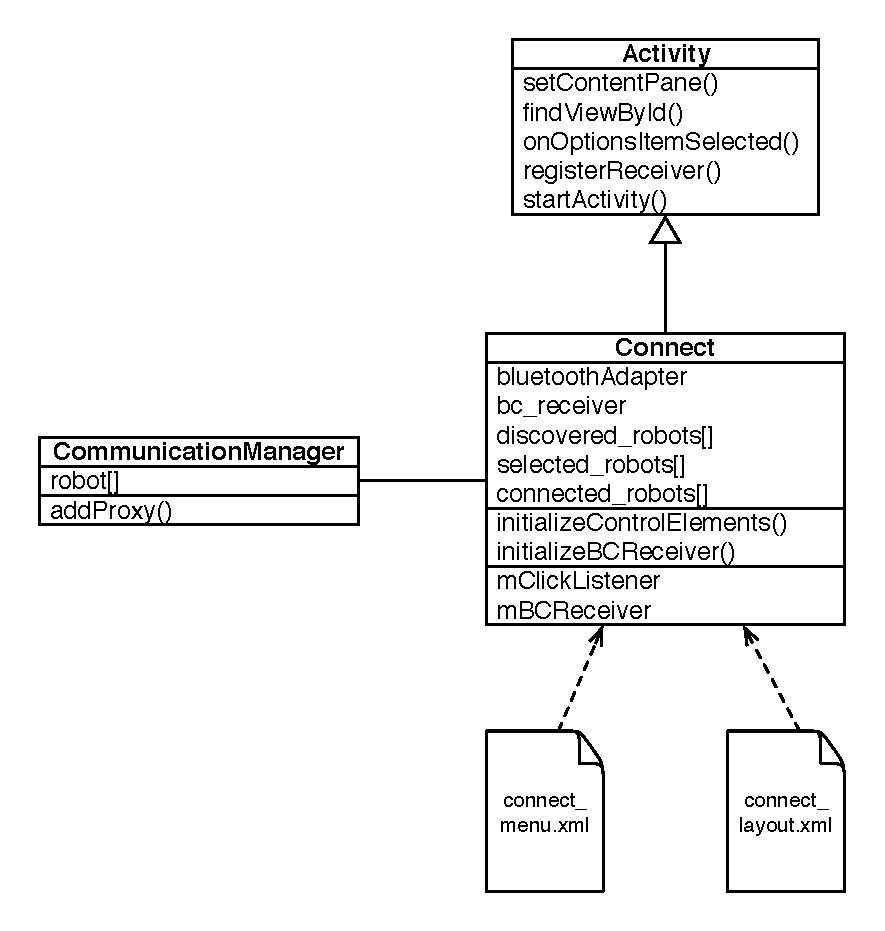
\includegraphics[width=10cm]{images/entwurf_connect.eps}
  			\caption{Klassendiagramm - Dialog `Connect'}
  			\label{fig:dialog_connect}
  	\end{figure}
	
	\paragraph*{Kurzbeschreibung} Der Dialog `Connect' (Abbildung \ref{fig:dialog_connect}) ist der Einsprungspunkt der gesamten Anwendung. Er dient
	der Auswahl der an der Erkundung teilnehmenden e-puck Roboter. 
	
	\paragraph*{Bluetooth-Schnittstelle} Die Activity verwaltet eine Referenz auf einen \textit{""Blue\-tooth-A\-dap\-ter}, eine Klasse der Android
	eigenen Bluetooth-API. Mit diesem kann nach verbindungsbereiten Robotern gesucht werden. Gefundene Geräte werden über Broadcast-Nachrichten des
	Betriebssystems gemeldet. Deshalb ist ein \textit{Broadcast-Receiver} mit entsprechenden Nachrichtenfiltern zur Verarbeitung der Nachrichten
	erforderlich.
	Die Realisierung des Broadcast-Receivers erfolgt als innere Klasse der Activity. Dieser wird mit der Methode \textit{registerReceiver()} zusammen
	mit einem \textit{IntentFilter} registriert.
	Der \textit{IntentFilter} wird durch setzen der entsprechenden Eigenschaft auf die beiden Ereignisse `Suche abgeschlossen' und `Gerät gefunden'
	eingestellt. Eingehende Nachrichten werden in der \textit{onReceive()}-Methode des Broadcast-Receivers verarbeitet.
	
	\paragraph*{Bluetooth-Suche} Beim erstmaligen Aufruf des Dialogs wird automatisch eine Suche nach verbindungsbereiten e-pucks gestartet. 
	Gefundene Roboter werden gespeichert (found\_robots) und mit ihren Bluetooth-Namen in einer ListView aufgelistet. Durch eine 
	Filterfunktion wird sichergestellt, dass nur e-puck Roboter angezeigt werden, die der im Pflichtenheft spezifizierten Namenskonvention genügen.
	Durch den Button 'New Search' hat der Benutzer die Möglichkeit, eine neue Suche zu starten. 
	
	\paragraph*{Auswahl der teilnehmenden e-puck Roboter} Durch Klick bzw. bei Touch auf die Einträge der ListView können diejenigen e-pucks
	ausgewählt werden, die an der Erkundung teilnehmen sollen. Ausgewählte Roboter bzw. deren Einträge erscheinen in grüner Schrift, nicht
	ausgewählte in roter Schrift. Ausgewählte Roboter werden gespeichert (selected\_robots).
	
	\paragraph*{Verbindungsherstellung}
	Bei Auswahl des Menüeintrags `Connect' wird die Anzeige des Dialogs solange gesperrt, bis zu allen ausgewählten e-pucks eine Bluetooth-Verbindung
	hergestellt wurde. Die Verbindungsherstellung erfolgt sequentiell. Jede erfolgreiche Verbindung liefert einen \textit{BluetoothSocket} zurück.
	Diese werden in einer Liste gesammelt bis alle Verbindungen aufgebaut wurden.
	
	\paragraph*{Erzeugung der RealPucks}
	Anschließend wird dem \textit{Environment} für jeden Socket eine neue Instanz der \textit{RealPuck}-Klasse hinzugefügt und der Dialog `Map' über
	eine \textit{Intent}-Nachricht gestartet.
	
	\paragraph*{Verhalten im Fehlerfall}
	Tritt während der Verbindungsherstellung ein Fehler auf (zum Beispiel e-puck ist nicht mehr verfügbar nachdem die letzte Suche beendet worden
	ist), wird die Herstellung der Verbindungen abgebrochen. Bereits aufgebaute Verbindungen werden beendet. Der Benutzer erhält eine entsprechende
	Hinweismeldung und hat die Möglichkeit eine neue Suche zu starten.
	
	\subsection*{Dialog `Simulation'}
	\label{subsec:dialog_sim}
	
	\begin{figure}[h]
			\centering
			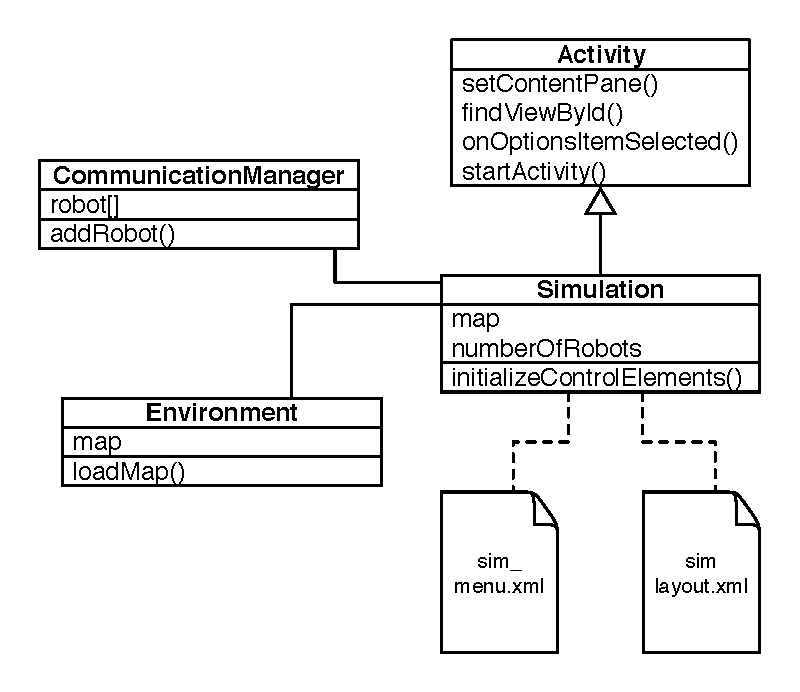
\includegraphics[width=10cm]{images/entwurf_sim.eps}
  			\caption{Klassendiagramm - Dialog `Simulation'}
  			\label{fig:dialog_sim}
  	\end{figure}
	
	\paragraph*{Kurzbeschreibung} Der Dialog `Simulation' (Abbildung \ref{fig:dialog_sim}) ermöglicht die Ausführung der Anwendung im
	Simulationsmodus. Sie bietet Funktionen zum Laden einer vordefinierten Karte und zum Festlegen der Anzahl der teilnehmenden virtuellen Roboter.
	
	\paragraph*{Auswahl und Laden einer vordefinierten Karte} Mit Hilfe des Button `Import' kann eine vordefinierte Karte aus dem Dateisystem des
	Smartphones ausgewählt und geladen werden. Die abgespeicherte Karte wird anschließend in eine \textit{GridMap} konvertiert und im Attribut
	\textit{map} temporär gespeichert.
	
	\paragraph*{Festlegung der Anzahl der teilnehmenden Roboter}
	Mit Hilfe eines ""Drop\-Down-Steu\-er\-ele\-ments kann der Benutzer die Anzahl der teilnehmenden e-puck Roboter festlegen. Die Maximalzahl
	beträgt sechs. Die Anzahl wird temporär in der Variablen \textit{numberOfRobots} gespeichert.
	
	\subsection*{Dialog `Map'}
	\label{subsec:dialog_map}
	
	\begin{figure}[h]
			\centering
			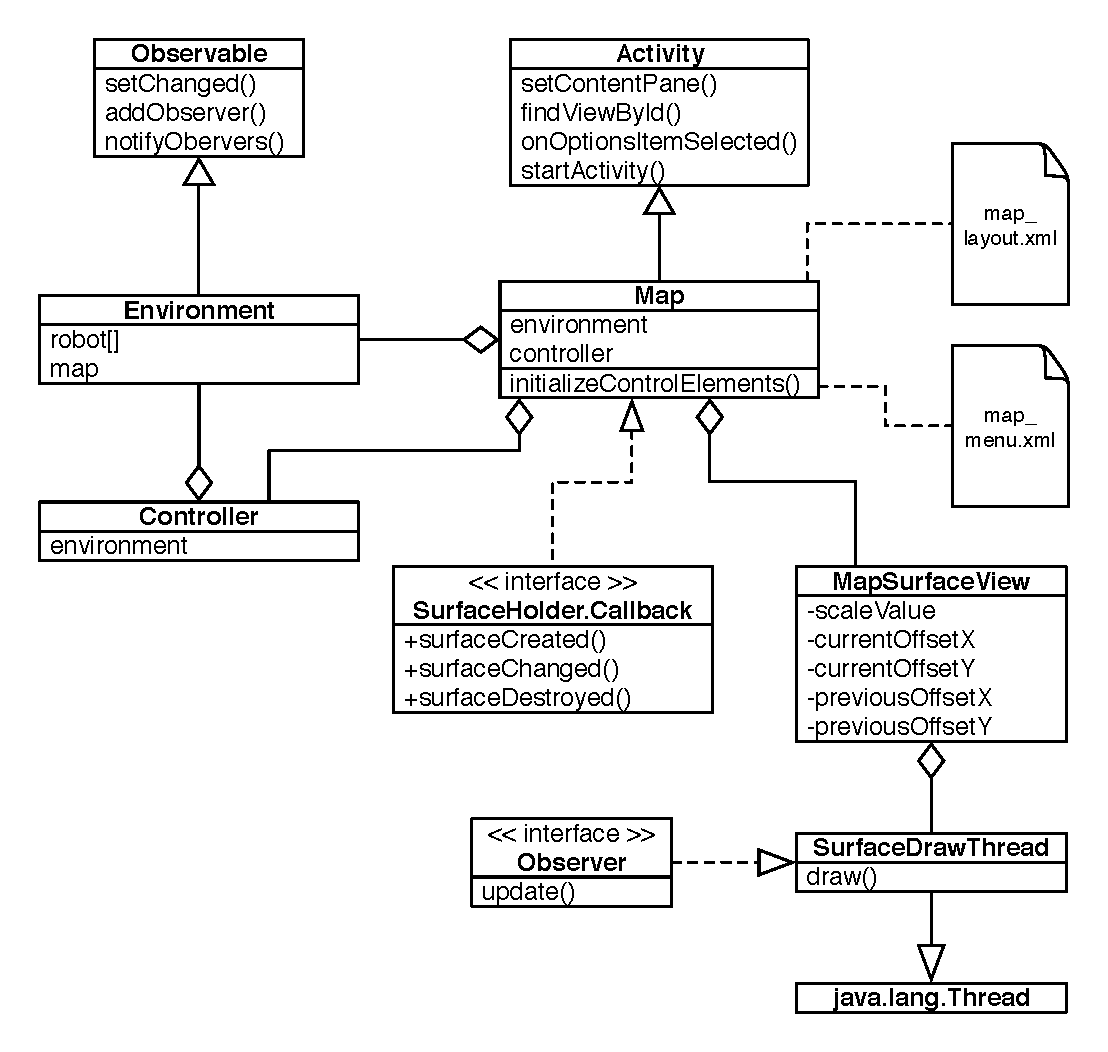
\includegraphics[width=10cm]{images/entwurf_map.eps}
  			\caption{Klassendiagramm - Dialog `Map'}
  			\label{fig:dialog_map}
  	\end{figure}
	
	\paragraph*{Kurzbeschreibung} Der Dialog `Map' (Abbildung \ref{fig:dialog_map}) stellt das bereits erkundete Gebiet und die Positionen der
	Roboter grafisch dar. Zusätzlich werden die Felder der Karte je nach Häugfigkeit der Befahrung unterschiedlich transparent dargestellt.
	
	\paragraph*{Zeichnung der Karte und der Roboterpositionen}
	Die Darstellung erfolgt mit Hilfe der Klasse \textit{MapSurfaceView}, die von der Klasse \textit{SurfaceView} der Android-API erbt. Diese Klasse
	bietet eine spezielle Zeichenoberfläche an, die durch einen zweiten Thread verwaltet wird. Das Zeichnen der Karte auf diese Oberfläche erfolgt
	asynchron zum normalen Layout-Prozess des Android Systems durch eine Instanz der Klasse \textit{SurfaceDrawThread}.
	Dieser enthält Methoden, um alle möglichen Knotentypen und Roboter an bestimmten Koordinaten zu zeichnen.
	
	\paragraph*{Autoskalierung der Karte}
	Im Lauf der Erkundung vergrößert sich die Karte ständig und wird möglicherweise zu groß, um auf dem Display komplett angezeigt zu werden.
    Die maximale Ausdehnung der Karte kann mit Hilfe der \textit{GridMap} des \textit{Environment} berechnet werden. Diese stellt den größten und
    kleinsten x-Wert und y-Wert zur Verfügung. Über den Skalierungsfaktor kann dann die Größe der Karte in Pixel berechnet werden. Der
    Skalierungswert stellt die Größe eines zu zeichnenden Knoten dar. Ein Knoten entspricht einer normalen Kreuzung, einer T-Kreuzung oder
    einer Ecke.
	Sollte die zu zeichnende Karte größer sein als das Display, so wird über die Funktion \textit{autoscale()} der Skalierungsfaktor verkleinert.
	Dadurch wird die Größe der zu zeichnenden Knoten reduziert und die Karte kann vollständig auf dem Display angezeigt werden. 
	
	\paragraph*{Scrollfunktion der Karte}
	Unterschreitet der Skalierungsfaktor einen bestimmten Schwellwert, findet keine Autoskalierung mehr statt, da die Darstellung sonst zu klein
	werden würde. Statt dessen wird die Karte scrollbar. Der angezeigte Kartenausschnitt kann dann durch Bewegung eines Fingers auf dem Touch-Screen
	verschoben werden.
	Die Verarbeitung der Touch-Events erfolgt in einem \textit{OnTouchListener} unter Verwendung der vier Offset-Werte. previousPositonX und
	previousPositionY speichern die Position des Fingers vor, currentPositonX und currentPositionY nach der Verschiebebewegung. Aus diesen Werten
	wird die Verschiebung des Kartenausschnitts berechnet.
	
	\paragraph*{Auswahl eines Roboters} Der Benutzer kann über ein ""Drop\-Down-Steu\-er\-ele\-ment einen teilnehmenden Roboter auswählen. Dieser
	wird auf der Karte besonders hervorgehoben. Außerdem werden die von ihm befahrenen Felder farbig gekenntzeichnet und ja nach Häufigkeit der
	Befahrung unterschiedlich transparent dargestellt. \\
	Die Auswahl des Roboters kann alternativ durch Touch auf die Darstellung des Roboters in der Karte erfolgen. Der Roboter wird dann im
	DropDown-Steuerelement als aktuelle Auswahl eingestellt. \\
	Soll kein Roboter ausgewählt werden, bietet das ""Drop\-Down-Steu\-er\-ele\-ment den Eintrag `none' an. \\ 
	Die Auswahl eines Roboters ist erst nach erfolgreicher Lokalisierung möglich. Wurde der Dialog durch die Import-Funktion aufgerufen, so ist keine
	Auswahl möglich. Das ""Drop\-Down-Steu\-er\-ele\-ment wird in diesen Fällen ausgegraut dargestellt.
	
	\paragraph*{Verhalten bei Verbindungsverlust} Verliert einer der e-puck Roboter die Verbindung zum Smartphone, so erhält der Benutzer eine
	entsprechende Hinweismeldung. Durch die Entfernung des zugehörigen RealPucks aus dem \textit{Environment} ist gewährleistet, dass der Roboter aus
	dem ""Drop\-Down-Steu\-er\-ele\-ment entfernt und nicht mehr auf der Karte dargestellt wird. War der ausgefallene e-Puck gerade ausgewählt, wird
	am ""Drop\-Down-Steu\-er\-ele\-ment der Eintrag `none' eingestellt.

	\subsection*{Dialog `Steer'}
	
	\begin{figure}[h]
			\centering
			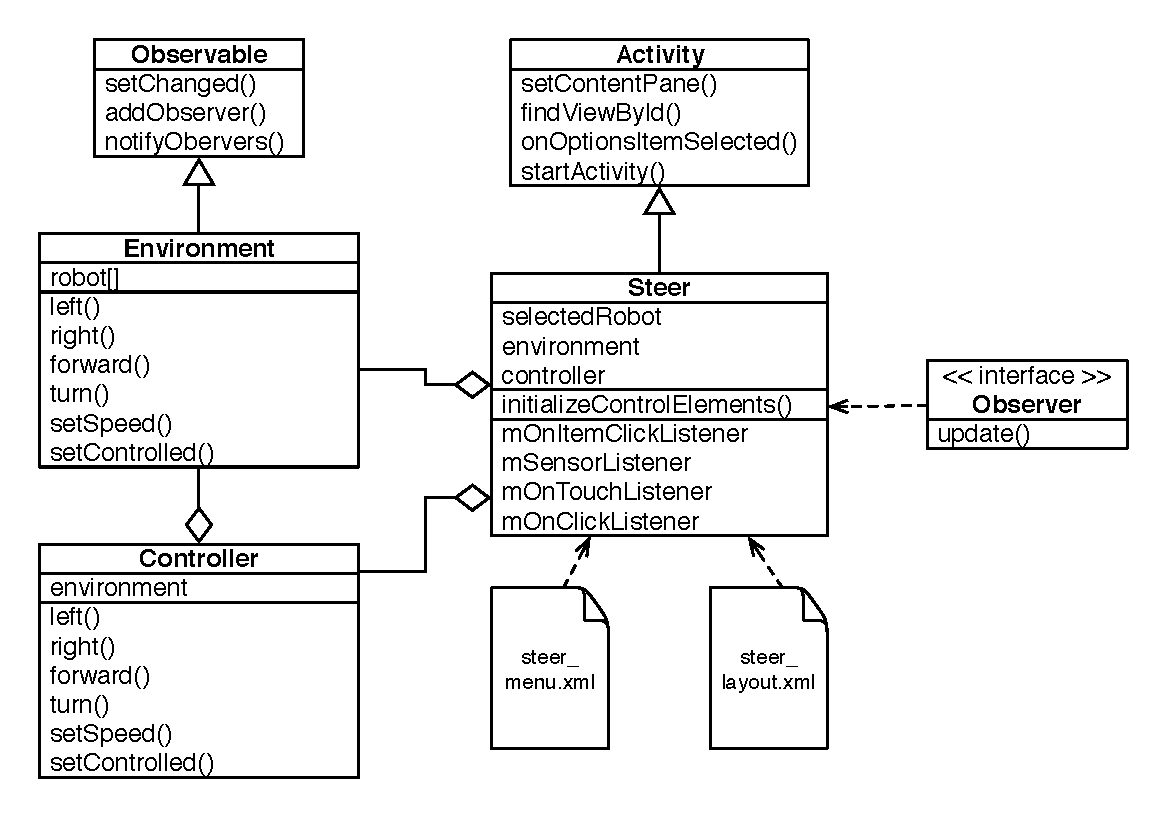
\includegraphics[width=10cm]{images/entwurf_steer.eps}
  			\caption{Klassendiagramm - Dialog `Steer'}
  			\label{fig:dialog_steer}
  	\end{figure}
	
	\paragraph*{Kurzbeschreibung}
	Der Dialog `Steer' (Abbildung \ref{fig:dialog_steer}) bietet die Möglichkeit, einen teilnehmenden Roboter auszuwählen und manuell zu steuern. Der 
	Benutzer kann den Roboter mit der 
	Steuerung geradeaus bewegen, um 90 Grad rechts und links herum drehen oder durch Drehung um 180 Grad wenden lassen. Der Roboter bewegt sich dabei
	weiterhin nur auf den Linien des Spielfeldes. \\
	Der Aufruf des Dialogs ist erst nach Abschluss des Lokalisierungsvorgangs der Roboter möglich.
	
	\paragraph*{Auswahl eines Roboters}
	Über ein ""Drop\-Down-Steu\-er\-ele\-ment kann der zu steuernde Roboter ausgewählt werden. Die ID des ausgewählten Roboters wird gespeichert.
	
	\paragraph*{Aktivierung/Deaktivierung der Steuerung} Durch Klick auf den Button `Start' wird die manuelle Steuerung aktiviert. Der entsprechende
	\textit{RealPuck} wird in den Zustand `CONTROLLED' versetzt und kann durch das von ihm implementierte Interface \textit{IRobot} gesteuert werden.
	Wird im ""Drop\-Down-Steu\-er\-ele\-ment `none' ausgewählt, kann die Steuerung nicht aktiviert werden. \\ \\
	Die Beschriftung des Buttons ändert sich nach Aktivierung auf `Stop'. Durch einen erneuten Klick auf die Schaltfläche kann die manuelle Steuerung
	deaktiviert werden. Der Roboter verlässt daraufhin den Zustand `CONTROLLED' und fährt mit seinem letzten Verhalten fort.
	
	\paragraph*{Auswahl der Steuerungsart} Ein weiteres ""Drop\-Down-Steu\-er\-ele\-ment ermöglicht die Auswahl der zu verwendeten Steuerungart. Zur
	Auswahl stehen die Steuerung über einen On-Screen-Joystick oder eine Kippsteuerung über den im Smartphone eingebauten Beschleunigungssensor.
	
	\paragraph*{Realisierung des On-Screen-Joysticks} Die Realisierung des On-Screen-Joystick geschieht durch einen einfachen \textit{onTouch}- bzw.
	\textit{""on\-Click\-E\-vent\-List\-e\-ner}. Berührt der Benutzer einen der vier möglichen Richtungsbuttons, so wird durch einen registrierten
	Listener das entsprechende Kommando über den globalen \textit{Controller} und das \textit{Environment} an den ausgewählten \textit{RealPuck}
	weitergeleitet.
	
	\paragraph*{Realisierung der Kippsteuerung} Die Realisierung der Steuerung mit den Beschleunigungssensoren erfolgt ähnlich: Statt der 
	\textit{onTouch}- bzw. \textit{""on\-Click\-E\-vent\-List\-e\-ner} wird ein \textit{SensorEventListener} der Android-API verwendet. Dieser wird
	an einem \textit{SensorManager} registriert und berechnet aus den aktuellen Sensormesswerten eine passende Richtungsanweisung. Diese wird über
	den globalen \textit{Controller} an den ausgewählten \textit{RealPuck} weitergegeben.
	
	\paragraph*{Weitergabe der Steuerungsbefehle an den e-puck} Wurde eine Richtungsanweisung an den \textit{RealPuck} weitergeleitet, so wird diese vom
	\textit{RealPuck} bzw. dem zugehörigen \textit{LogicThread} per Bluetooth an den e-puck weitergegeben. Dieser sendet nach Ausführung eine
	Bestätigungsnachricht.
	Solange die Bestätigungsnachricht nicht eingegangen ist, werden keine weiteren Richtungsanweisungen mehr an den Roboter weitergegeben. In der 
	Zwischenzeit gegebene Anweisungen werden außerdem gespeichert.
	
	\paragraph*{Einstellung der Geschwindigkeit} Die Einstellung der Geschwindigkeit erfolgt in beiden Fällen über ein Slider-Steuerelement. Die
	Weitergabe von Geschwindigkeitsanweisungen erfolgt ebenfalls über einen \textit{OnClickListener}, der die einzustellende Geschwindigkeit an den
	globalen \textit{Controller} und das \textit{Environment} weiter gibt.
	
	\paragraph*{Verhalten bei Verbindungsverlust} Tritt während der Steuerung ein Fehler durch den Verlust der Verbindung zum e-puck auf, so wird die
	manuelle Steuerung deaktiviert. Der Benutzer erhält eine entsprechende Hinweismeldung. Der Roboter wird aus dem DropDown-Steuerelement entfernt.
	Statt dessen wird `none' eingestellt.
		
	\subsection*{Dialog `Statistics'}
	
	\begin{figure}[h]
			\centering
			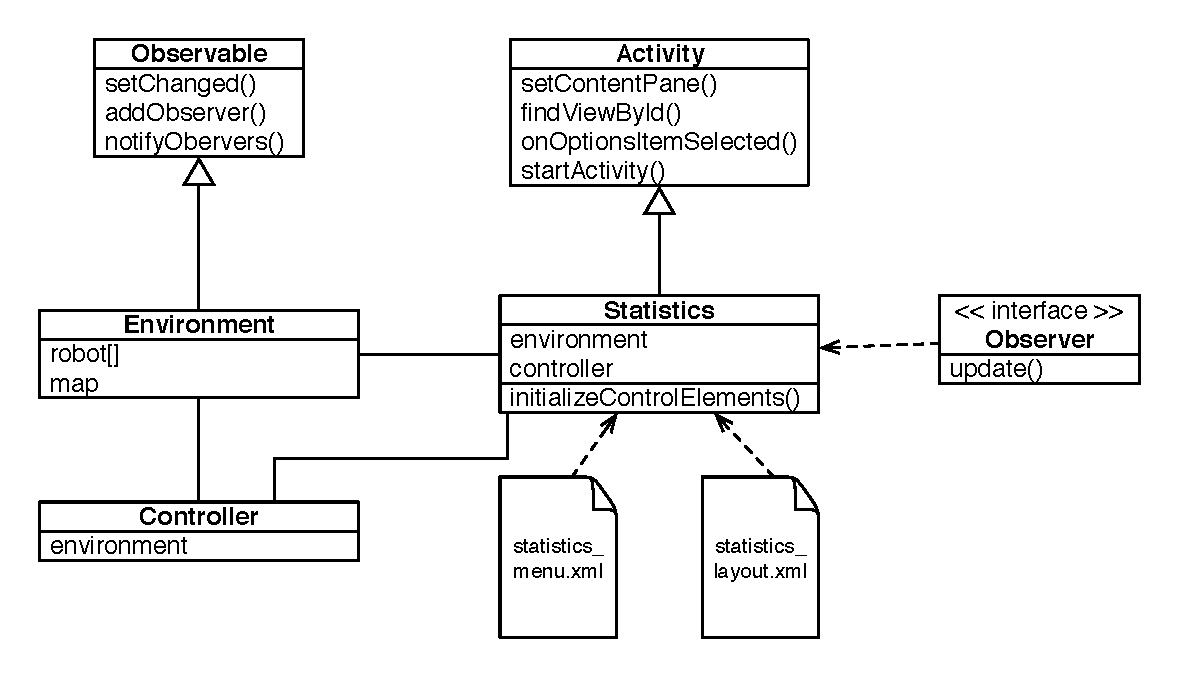
\includegraphics[width=10cm]{images/entwurf_statistics.eps}
  			\caption{Klassendiagramm - Dialog `Statistics'}
  			\label{fig:dialog_statistics}
  	\end{figure}
	
	\paragraph*{Kurzbeschreibung} Der Dialog „Statistics“ bietet dem Benutzer die Möglichkeit, Statistiken zum aktuellen Erkundungsverlauf zu
	betrachten.
	
	\paragraph*{Angezeigte Statistiken} Nach Start des Dialogs werden folgende Informationen zum aktuellen Erkundungsverlauf angezeigt:
	\begin{itemize}
	\item die Zahl der bisher erkundeten Knoten je Roboter
	\item die Zahl der bisher befahrenen Knoten je Roboter
	\item die Gesamtzahl der bisher erkundeten Knoten
	\item die Gesamtzahl der bisher befahrenen Knoten
	\item das Verhältnis der beiden Gesamtzahlen
	\end{itemize}
	
	\paragraph*{Verhalten bei Verbindungsverlust} Tritt während der Steuerung ein Fehler durch den Verlust der Verbindung zum e-puck auf, so erhält
	 der Benutzer eine entsprechende Hinweismeldung.        
      		
		\subsection{Repräsentation der e-puck Roboter}
			\label{sec:repraesentation}
			\begin{figure}[h]
				\centering
				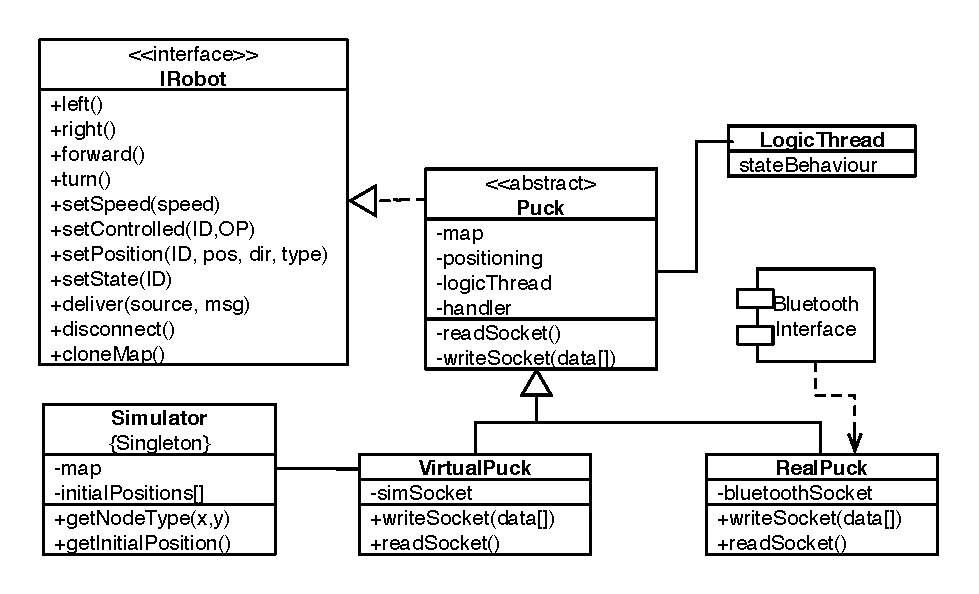
\includegraphics[width=10cm]{images/android_puck.eps}
  				\caption{Repräsentation der e-puck Roboter}
  				\label{fig:puck}
  			\end{figure}		
      		Die Repräsentation der Roboter auf dem Handy wird über das Interface \textit{IRobot} an den \textit{CommunicationManager} angebunden.
      		Damit lassen sich verschiedene konkrete Roboter durch die Anwendung darstellen.\\
      		Die Erkundung von Spielfeldern kann neben der Verwendung von realen e-puck Robotern auch per Simulation auf dem Smartphone durchgeführt
      		werden. Dafür wählt der Benutzer beim Start-Dialog (Activity \textit{Import}) eine bereits exportierte Karte und die Anzahl der virtuellen
      		e-pucks. Je nach Art der Erkundung werden die notwendigen Instanzen der Klasse \textit{VirtualPuck} (virtueller e-puck) oder Klasse \textit{RealPuck}
      		(realer e-puck)	erstellt und am Kommunikationsmanager registriert. Beide Klassen erben von der abstrakten Klasse \textit{Puck}, welche Basis-Funktionen
      		der e-puck-Repräsentationen beinhaltet.  Sie enthält Zustandsdaten wie zum Beispiel die lokale Karte oder den Zustand der Roboter-Repräsentationen.
      		Im gesamten Dokument werden \textit{RealPucks} zur Erläuterung verwendet.
      		\textit{Puck} implementiert das Interface \textit{IRobot} und enthält als Attribut eine Instanz der Klasse \textit{LogicThread}, der für die Verarbeitung von
      		Fahrplanungen zuständig ist. Der Informationsaustausch zwischen (realen oder virtuellen) e-pucks bezüglich Knotenerkennung wird über die Methdoen
      		\texttt{readSocket()} bzw. \texttt{writeSocket(data[])} durchgeführt.\\
      		\paragraph*{RealPuck}      	
			Die \textit{RealPuck}-Klasse ist die Repräsentation der realen e-puck Roboter auf dem Smartphone. Als Socketanbindung verwenden sie eine Bluetooth-
			Schnittstelle. Diese hält eine Verbindung zum realen e-puck.
			\paragraph*{VirtualPuck}
			Die Klasse \textit{VirtualPuck} ist für die Simulation der Roboter auf dem Smartphone gedacht. Sie verwenden anstatt einer Bluetooth-Verbindung einen
			``Socket'' zur Klasse \textit{Simulator}. Diese Klasse simuliert sämtliche Nachrichten, die im realen Durchlauf Roboter gesendet hätte. Durch diese
			Vorgehensweise kann die selbe Logik für virtuelle sowie reale Repräsentationen verwendet werden.
			\paragraph*{Aufgaben des \textit{LogicThread}}
		\begin{itemize}
			\item Nachrichtenaustausch mit dem e-puck \\
				Über den Socket werden Daten vom e-puck Roboter empfangen und gesendet.
			\item Senden von Broadcast-Nachrichten \\
				Mit Hilfe der \textit{broadcast()}-Methode der \textit{CommunicationManager}-Klasse können Nachrichten an alle
				Pucks sowie an das \textit{Environment} selbst übermittelt werden. \\
				Diese Nachrichten enthalten	Zustandsupdates, die für alle Teilnehmer relevant sind. Darunter fallen z.B.
				Positionsupdates, Kartenupdates oder Nachrichten der abstrakten Logik.
			\item Empfangen von Nachrichten  \\
				Nachricht werden über die \textit{deliver()}-Methode angenommen und durch das Chain-of-Responsibility-Pattern verarbeitet.
			\item Zustandsbeschreibung aller e-puck Roboter \\
				Mithilfe von \textit{Positioning}-Objekten wird der aktuelle Zustand aller e-puck Roboter lokal gespeichert.
			\item Verwaltung der lokalen Karte \\
				Die lokale \textit{GridMap} muss sowohl bei lokalen als auch bei Updates eines anderen e-pucks aktualisiert werden. 
			\item Umsetzung von Benutzereingaben \\
				Geschwindigkeitsänderungen sowie Fahrtanweisungen durch den Benutzer werden verarbeitet und gegebenenfalls
				an den e-puck weitergeleitet.
			\item Management der künstlichen Intelligenz \\
				Hierunter fällt die Anwendung der abstrakten Logik wie z.B. Erkundung und Kollisionsvermeidung. Diese Verhaltensweisen werden durch
				spezielle Verhaltensklassen (\textit{ConcreteBehaviour}) modelliert. Alle Verhaltensklassen implementieren das Interface
				\textit{IBehavoir}
		\end{itemize} 
  		
  		\subsection{Nachrichtenbehandlung}
  			Im Android-System wird das Chain-of-Responsibility-Pattern verwendet, um Nachrichten zwischen einem e-puck Roboter und einer
  			RealPuck, zwei RealPucks und zwischen RealPucks und dem Environment zu analysieren und zu verarbeiten. Die Grundidee hinter
  			diesem Pattern ist, dass die Nachricht durch eine Liste
  			von konkreten Handlerklassen, die von einer abstrakten Handlerklasse erben, gereicht wird und der richtige Handler die Nachricht
  			verarbeitet. Sobald eine Nachricht von einem Handler erkannt und bearbeitet wurde gibt er true zurück. Falls der Handler nicht
  			für die Nachricht verantwortlich ist, gibt er sie an den nächsten Handler weiter. Falls kein Handler die Nachricht verarbeitet, so wird
  			dem Aufrufer dies über den Rückgabewert `false' zurückgeliefert. Im Gegensatz zu herkömmlichen Nachrichtenbearbeitungen wird hier ein
  			hohes Maß an Flexibilität erreicht und das Hinzufügen eines neuen Nachrichtentyps wird erleichtert, da nur eine neue Klasse in die
  			Liste der Handler hinzugefügt werden muss. \\ \\
  			Vorteile:
  			\begin{itemize}
  				\item Unabhängigkeit zwischen Sender und Empfänger (Entkopplung)
  				\item Sehr gut erweiterbar, falls ein neuer Nachrichtentyp hinzugefügt werden soll
  				\item Mehrere Klassen kümmern sich um die Verarbeitung, d.h. die Fehlersuche und -behandlung wird vereinfacht
  				\item Größere Flexibilität bei der Bearbeitung von Nachrichten
  				\item Mithilfe des Rückgabewerts wird erkannt, ob eine Nachricht behandelt wurde
  			\end{itemize}  
  			Teilnehmer:
   			\begin{itemize}
  				\item Handler\\Definiert ein Interface für die Requests\\Besitzt eine Referenz auf den nächsten Handler bzw. eine \textit{Null}-Referenz
  					im Falle des letzten Handlers.
  				\item Konkrete Handler\\Größere Flexibilität bei der Bearbeitung von Nachrichten\\
  					Mithilfe des Rückgabewerts wird erkannt, ob eine Nachricht behandelt wurde
  				\item Receiver \\ Ruft Funktion handlerequest(Nachricht) auf ersten Listenelement der Handler auf
  			\end{itemize}   	
			\begin{figure}[h]
				\centering
				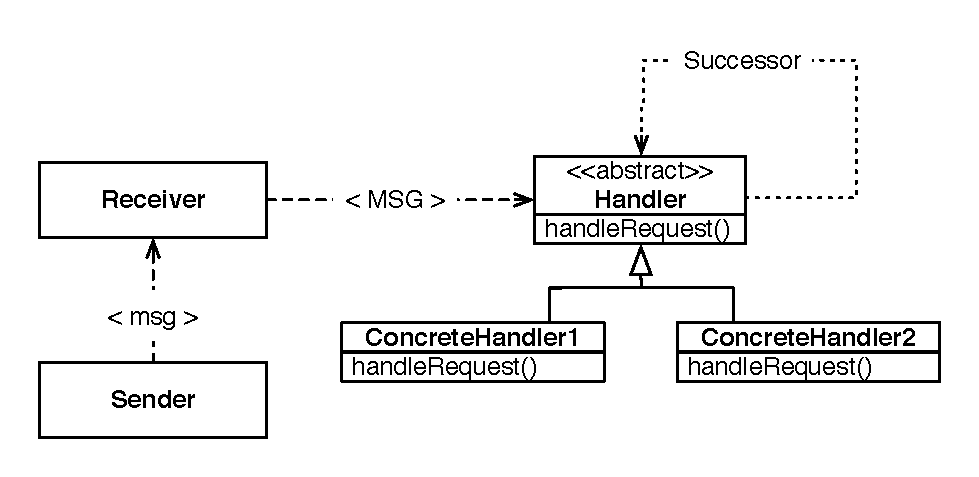
\includegraphics[width=10cm]{images/android_handler.eps}
  				\caption{Chain of Responsibility - Entwurfsmuster}
  			\end{figure}	
  			Erklärung der Abbildung:
   			\begin{enumerate}
  				\item Ein Sender schickt eine Nachricht an eine Empfängerklasse, die eine Liste aus konkreten Handlern,
  					welche von der abstrakten Klasse Handler erben, enthält.
  				\item Diese Klasse gibt die Nachricht an den ersten Handler seiner Liste weiter und ruft dort die Funktion handlerequest(Nachricht),
  					die den Rückgabetyp Boolean hat, auf.
  				\item Der Handler leitet die Nachricht an seinen direkten Nachfolger weiter und ruft dort wieder handlerequest(Nachricht) auf, sofern
  					er nicht für die Bearbeitung der Nachricht zuständig ist. In diesem Fall behandelt er die Nachricht entsprechend und gibt true zurück
  				\item Der Handler, der keinen Nachfolger mehr hat gibt den Wert false zurück. Somit weiß die Empfängerklasse dass für die Nachricht kein
  					entsprechender Handler zur Verfügung steht.  					
  			\end{enumerate}   

	\section{Abstrakte Logik}

	\subsection{A$^\ast$ Suchalgorithmus}
		\label{subsec:astern}
		\paragraph{Problemstellung}
			Damit die e-pucks ihre Ziele, wie zum Beispiel das Auffinden eines noch nicht erkundeten Knotens oder die 
			Rückkehr zur Startposition, möglichst effizient erreichen können, wird ein Pfadplanungsalgorithmus benötigt. 
			Dieser soll auf Grundlage einer bereits (teilweise) erkundeten Karte, einer Liste von möglichen Zielpunkten 
			und einer Startposition, eine Liste von Pfaden zu allen Zielen erstellen.\\
			Außerdem soll die Funktion zur Bewertung der tatsächlichen Knotenkosten austauschbar sein. Dadurch lässt 
			sich der Algorithmus für unterschiedliche Aufgaben verwenden.
		\paragraph{Überblick}
			A$^\ast$ ist ein informierter Offline-Suchalgorithmus, der einen optimalen Pfad zwischen zwei Knoten in kürzester 
			Laufzeit findet, falls dieser existiert. Alle Knoten werden mit einem der drei folgenden Typen 
			identifiziert, welche jedoch nur in diesem Kontext gültig sind:
			\begin{itemize}
				\item unbekannt: Zu diesem Knoten ist noch kein Pfad bekannt
				\item bekannt (open): Zu diesem Knoten ist ein (suboptimaler) Pfad bekannt
				\item erkundet (closed): Zu diesem Knoten ist ein optimaler Pfad bekannt
			\end{itemize}

			Jeder erkundete oder bekannte Knoten besitzt eine Referenz auf seinen Vorgänger. Diese Verkettung stellt den 
			Pfad zum Startknoten dar. Für erkundete Knoten ist dies auch der kürzeste Pfad. Außerdem besitzen alle 
			bekannten und erkundeten Knoten einen Wegkostenzähler. \\
			Der Container der bekannten Knoten verwendet einen Binary-Heap. Dieser ermöglicht das effiziente Entfernen
			des jeweils günstigsten als nächstes zu erkundenden Knotens. Der Schlüssel setzt sich dabei aus den 
			aktuellen Wegkosten zum Start und einer Schätzung der Wegkosten zum aktuellen Ziel zusammen. \\
			Der Container der erkundeten Knoten ist ein Binärbaum, um Suchoperationen zu beschleunigen.
		\paragraph{Wegkosten und Heuristik}
			Der Algorithmus verwendet eine Bewertungsfunktion, um eine Aussage über die möglichen Gesamtwegkosten eines 
			Knotens treffen zu können. Diese werden durch die Summe aus den tatsächlichen Wegkosten des Vorgängerknotens, 
			den Übergangskosten zum aktuellen Knoten und einer Schätzung der verbleibenden Kosten bis zum Ziel 
			errechnet. \\

			Die Funktion zur Berechnung der Übergangskosten \textit{calculateCosts()} ist austauschbar, wodurch sich das
			Verhalten des Algorithmus trimmen lässt. Es ist jedoch zu beachten, dass die tatsächlichen Kosten nie den
			Schätzwert unterschreiten dürfen. Damit z.B. eine Kollision aktiv vermieden wird, müssen die Kosten eines
			blockierten Knotens höher sein als die Kosten des kürzesten lokalen Umwegs. \\

			Als Schätzfunktion (Heuristik) wird hier die Absolutsummennorm verwendet. Mit Hilfe der Heuristik wird eine 
			zielgerichtete Knotenexpansion erreicht, da nur ein bekannter Knoten mit den 
			geringsten Gesamtkosten als nächstes analysiert wird.
		\paragraph{Datenstrukturen}
			Benötigt wird eine Knotenklasse \textit{AStarNode}, die eine Referenz auf einen Vorgängerknoten vom selben
			Typ sowie eine Referenz auf	einen Graphknoten \textit{MapNode} der Karte enthält. Außerdem enthält sie
			einen Integer, der die aktuellen Kosten bis zum Startknoten angibt.
		\paragraph{Interface}
			Es wird das Interface \textit{IPathFinder} von der Klasse \textit{AStarPathFinder} implementiert:
			\begin{itemize}
				\item \textit{AStarNode[] find(MapNode start, MapNode[] destinations)} führt eine Suche durch und
				gibt die kürzesten Pfade zurück
				\item \textit{int calculateCosts(MapNode from, MapNode to)} berechnet die Übergangskosten von einem
				Knoten zu einem angrenzenden Knoten.
			\end{itemize}
		\paragraph{Ablauf}
			Der Algorithmus basiert auf dem Buch ``Game Programming Gems''\footnote{Abschnitt ``Path Finding Strategies''},
			jedoch mit einer Erweiterung für die Suche mehrerer Zielknoten. Dazu wird nach jeder erfolgreichen Suche
			eines Zielknotens der Container der bekannten Knoten umsortiert, damit jeweils der günstigste Knoten für den
			nächsten Zielknoten extrahiert werden kann. Durch diese Modifikation muss die Berechnung nicht für jeden
			Zielknoten neu durchgeführt werden, da auf bereits berechnete Pfadabschnitte zurückgegriffen werden kann.

		\subsection{Erkundungsalgorithmus}
			Im Folgenden wird der Algorithmus für die Erkundung eines unbekannten Spielfeldes mit Hilfe kooperativer Roboter erläutert. Das
			Vorgehen ist ähnlich zu dem, das von Yamauchi	\footnote{Frontier-Based Exploration Using Multiple Robots, ACM Press, 1998}
			vorgeschlagen wurde. Es handelt sich hierbei um eine Logik, welche die Roboter in Grenzregionen zu unbekannten Gebieten führt.
			Der Ansatz verwendet dezentral gespeicherte Karteninformationen, welche alle Teilnehmer lokal speichern. Damit
			kann die Erkundung effizient ausgeführt werden und ist robust gegenüber Ausfälle einzelner Roboter.
			\paragraph*{Definition} Ein unbekannter Knoten wird definiert als Knoten, der noch nicht von einem e-puck Roboter befahren wurde
				sowie mindestens an einem und maximal an drei befahrenen Knoten angrenzt.
			\paragraph*{Bemerkung} Ein unbefahrener Knoten, der an vier befahrene Knoten angrenzt ist kein unbekannter Knoten.
			\paragraph*{Algorithmus}Für die Berechnung eines günstigsten unbekannten Knoten wird eine mehrschichtige Logik verwendet.
				Jede Ebene behandelt einen bestimmten semantischen Aspekt und hat Einfluss auf die letztendliche Auswahl des Zielknotens. Für
				jeden unbekannten Knoten wird eine Kennzahl berechnet, wobei der Knoten mit der kleinsten Zahl den günstigsten darstellt. Falls
				mehrere günstigste Knoten existieren, so entscheidet die Berechnungsreihenfolge. Die Ebenen berechnen abhängig von ihren Regeln
				ihre eigenen Summen und addieren sie zur globalen Summe hinzu.
				\subparagraph*{Ebene 0: Entfernung} Ein wichtiges Kriterium zum Bestimmen des günstigsten unbekannten Knoten ist dessen
					Entfernung zum Roboter. Diese Ebene wird vollkommen von dem \textit{A*-Algorithmus} 
					übernommen, welcher auch bei der Wegsuche verwendet wird (siehe Kapitel \ref{subsec:astern}).
  				\subparagraph*{Ebene 1: Restbereiche} Unbekannte Bereiche, die vollständig innerhalb von erkundeter Gebiete liegen, werden vom
  					Algorithmus als weniger 'attraktiv' angesehen. Somit wird erreicht, dass potentiell große, unbekannte Teile der Karte
  					bevorzugt erkundet werden. \\
  					Es wird ein naives und statisches Vorgehen für die Logik verwendet. Es wird festgestellt, welche unbekannte Knoten sich innerhalb
  					eines vollständig erkundeten Bereiches befinden. Diesem Knoten wird der Wert 1 hinzu addiert (siehe Abbildung \ref{fig:level1}).  			
					\begin{figure}[h]
						\centering
						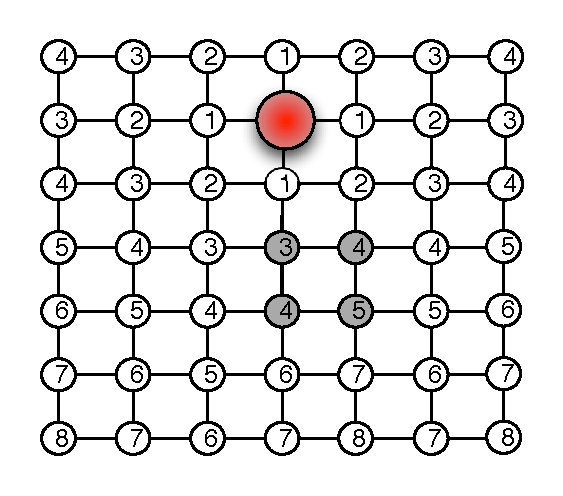
\includegraphics[width=10cm]{images/eingeschlossen.eps}
  						\caption{Unbekannte Bereiche innerhalb erkundeter Gebiete}
  						\label{fig:level1}
  					\end{figure}
  				\subparagraph*{Ebene 2: Gemeinsame Erkundung} Ziel dieser Ebene ist es, dass verschiedene unbekannte Gebiete möglichst von
  					wenigen Robotern gleichzeitig erkundet werden. Damit lässt sich doppelte Arbeit einsparen und die Effektivität steigern.\\
  					Die Logik verwendet zur Verarbeitung die Information anderer Roboter. Diese senden Broadcast-Nachrichten, sobald ein zu erkundender
  					Knoten festgelegt wurde. Die benachbarten unbekannten Knoten werden damit automatisch für die weitere Erkundung anderer e-pucks
  					weniger interessant. Der unbekannte Knoten an sich erhält zusätzlich	5 	Punkte, einem benachbarten Knoten werden 4 Punkte hinzu
  					addiert usw. bis zum 4. Nachbar, welcher noch einen Punkt zusätzlich erhält. Zur Berechnung der Nachbarn wird die Absolutsummennorm
  					verwendet:
					\begin{eqnarray}
						||x|| = \sum_{j=1}^n |x(j)|
					\end{eqnarray}
					Im zweidimensionalen Fall lautet die Norm: $||(x,y)||=|x| + |y|$. Falls Hindernisse oder unbekannte Gebiete auf Fahrlinien zwischen
					zwei Punkten liegen, so dieser direkte Weg ignoriert (siehe Abbildung \ref{fig:level1}). 			
					\begin{figure}[h]
						\centering
						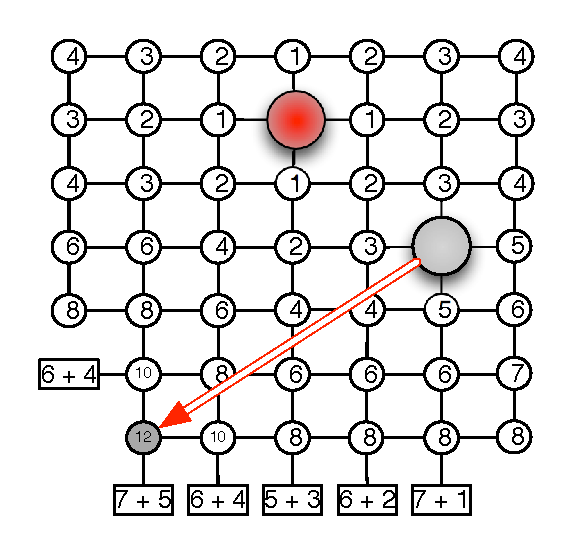
\includegraphics[width=10cm]{images/kooperation.eps}
  						\caption{Gemeinsame Erkundung von 2 Robotern}
  						\label{fig:level2}
  					\end{figure} 
  				\subparagraph*{Klassen-Entwurf} Um eine einfache Erweiterbarkeit der Logik-Ebenen zu erreichen, werden diese in Form einer
  					verketteten Liste von Logik-Instanzen realisiert. Eine Logik Klasse implementiert hierbei das Interface \textit{Exploration}, welches
  					die Methode \textit{execute} enthält. In dieser Methode werden die Knotenwerte entsprechend zu den jeweiligen Logik-Ebenen
  					addiert. Die Karte wird in Form von Knotenwerte übergeben, der Rückgabewert ist die Koordinate des günstigsten Knoten.
 					\begin{figure}[h]
						\centering
						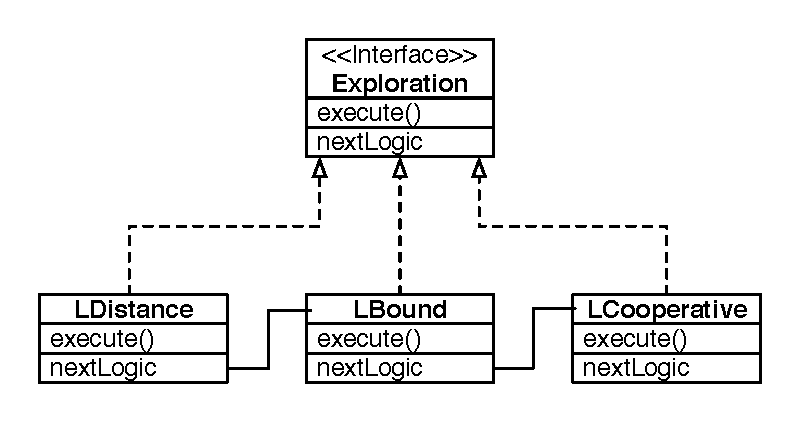
\includegraphics[width=10cm]{images/exploration_design.eps}
  						\caption{Klassenmodell des Erkundungsalgorithmus}
  						\label{fig:klassen_modell}
  					\end{figure} 
		\subsection{Lokale Lokalisierung}
			Die lokale Lokalisierung wird verwendet, um lokal Karten- sowie Positionsinformationen zwischen den
			e-puck Robotern auszutauschen. In anderen Worten, die e-pucks sollen ihre gegenseitige Lage kennen und sich auf ein einheitliches
			Koordinatensystem einigen. Für die Synchronisation werden die äußeren Abstandssensoren verwendet. Wie im Pflichtenheft definiert,
			werden bei dieser Lokalisierungsart alle Roboter auf zusammenhängenden Knoten aufgestellt.
			 \begin{figure}[h]
				\centering
				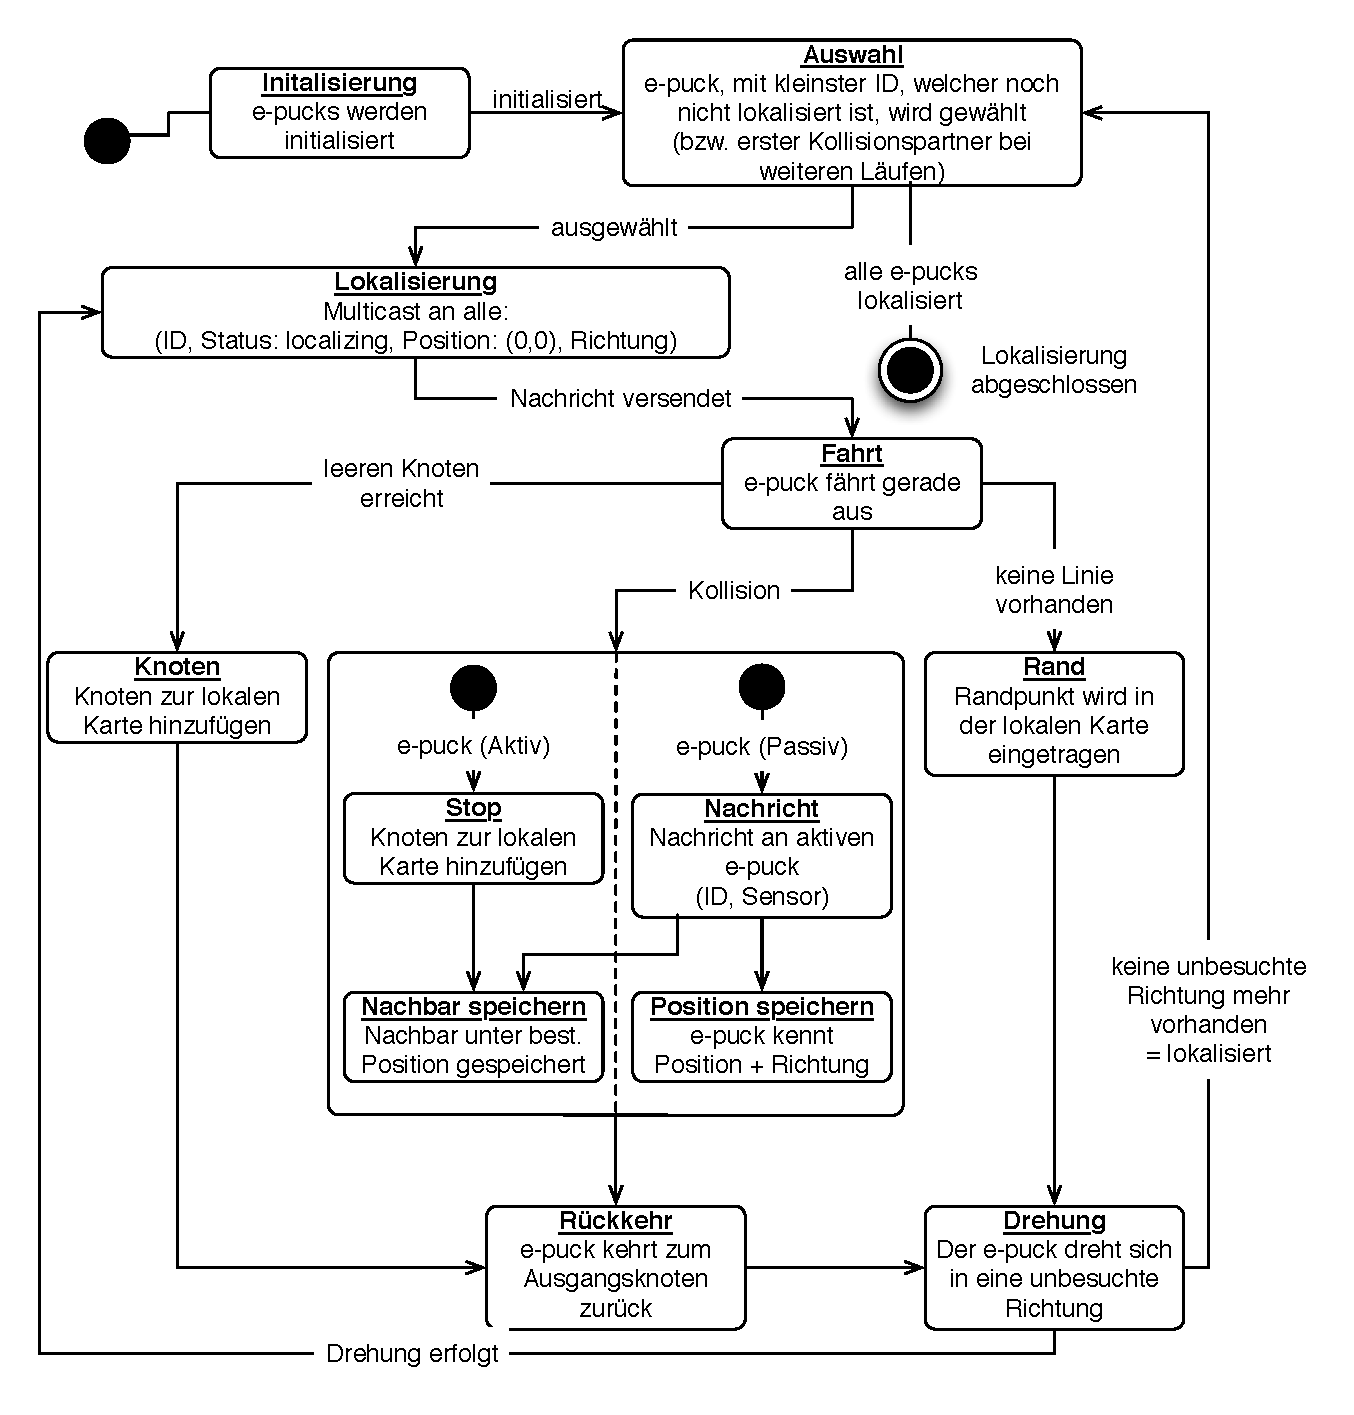
\includegraphics[width=10cm]{images/lokale_lokalisierung.eps}
  				\caption{Zustandsdiagramm - Algorithmus zur lokalen Lokalisierung}
  				\label{fig:lokale_lokalisierung}
  			\end{figure}
			Bei dem Algorithmus (siehe Abbildung \ref{fig:lokale_lokalisierung}) durchläuft jeder Roboter einzeln einen Synchronisierungslauf, in Reihenfolge ihrer IDs.
			Zunächst sendet der ausgewählte e-puck an alle Teilnehmer eine Nachricht, mit der er sein Lokalisierungsvorhaben ankündigt.
			Anschließend fährt er in gerader Richtung bis einer der folgenden Fälle eintritt:
			\begin{enumerate}
				\item Ein leerer Knoten wurde erreicht \\
				$\Longrightarrow$ Der Knoten wird zur lokalen Karte des e-pucks hinzugefügt und zum Ausgangsknoten zurückgekehrt.
				\item Eine Kollision ist aufgetreten \\
				$\Longrightarrow$ Der Knoten wird zur lokalen Karte des e-pucks hinzugefügt. Der passive Kollisionspartner sendet eine
				Nachricht an den aktiven Roboter und speichert seine Position bzw. Richtung  (die ID und Position weiß er durch die Ankündigung).
				Der aktive e-puck speichert seinen Nachbar und fährt zurück zum Ausgangsknoten.
				\item Es wird keine Linie erkannt \\
				$\Longrightarrow$ Es wird ein Randpunkt in die lokale Karte hinzugefügt.
			\end{enumerate}
			Sobald der aktive Roboter zurück bzw. noch immer am Ausgangsknoten ist, wird eine Drehung in eine bisher unerkundete Richtung
			durchgeführt. Sollte eine solche existieren, beginnt der e-puck erneut mit der Erkundung wie vorhin. Sollte keine Richtung mehr zu
			erkunden sein, so ist der Roboter lokalisiert. Der Partner, welcher die erste Kollision hervorgerufen hat und noch nicht lokalisiert ist,
			wird verwendet um den selben Lokalisierungsprozess durchzuführen. Dabei können bereits bekannte Richtungen vorhanden sein und
			ignoriert werden.\\ \\
			Dieser Wechsel wird solange wiederholt, bis sämtliche Roboter lokalisert sind ist.
		\subsection{Globale Lokalisierung}
			Die lokale Lokalisierung ist nur dann einsetzbar, falls alle Roboter auf angrenzenden Knoten stehen. Für die Wunschfunktion,
			bei der die e-pucks auf beliebigen Knoten des Spielfeldes starten können, ist es notwendig eine globale Lokalisierung
			durchzuführen. \\
			Dieses Vorhaben soll möglichst deterministisch ablaufen, sodass keine Spielfeld-bedingten Ausnahmen auftreten können. Daher ist das
			erste Ziel jedes Teilnehmers, den Rand des Spielfeldes zu erreichen. Sobald er dies erkannt hat, wird eine Nachricht an alle anderen
			gesendet und gewartet bis sämtliche Roboter diesen Rand erreicht haben. Zu diesem Zeitpunkt beginnt der e-puck mit der niedrigsten
			ID die Umrandung des Spielfeldes, bis die erste Kollision mit einem Teilnehmer geschieht. Der aktive Roboter fährt zum letzten Knoten
			und beendet die Umrundung. Dafür beginnt der Kollisionspartner sich auf die Suche nach dem nächsten Teilnehmer zu machen. Die 
			Lokalisierung findet ähnlich zu Abbildung \ref{fig:lokale_lokalisierung} statt.
		 	\begin{figure}[h]
				\centering
				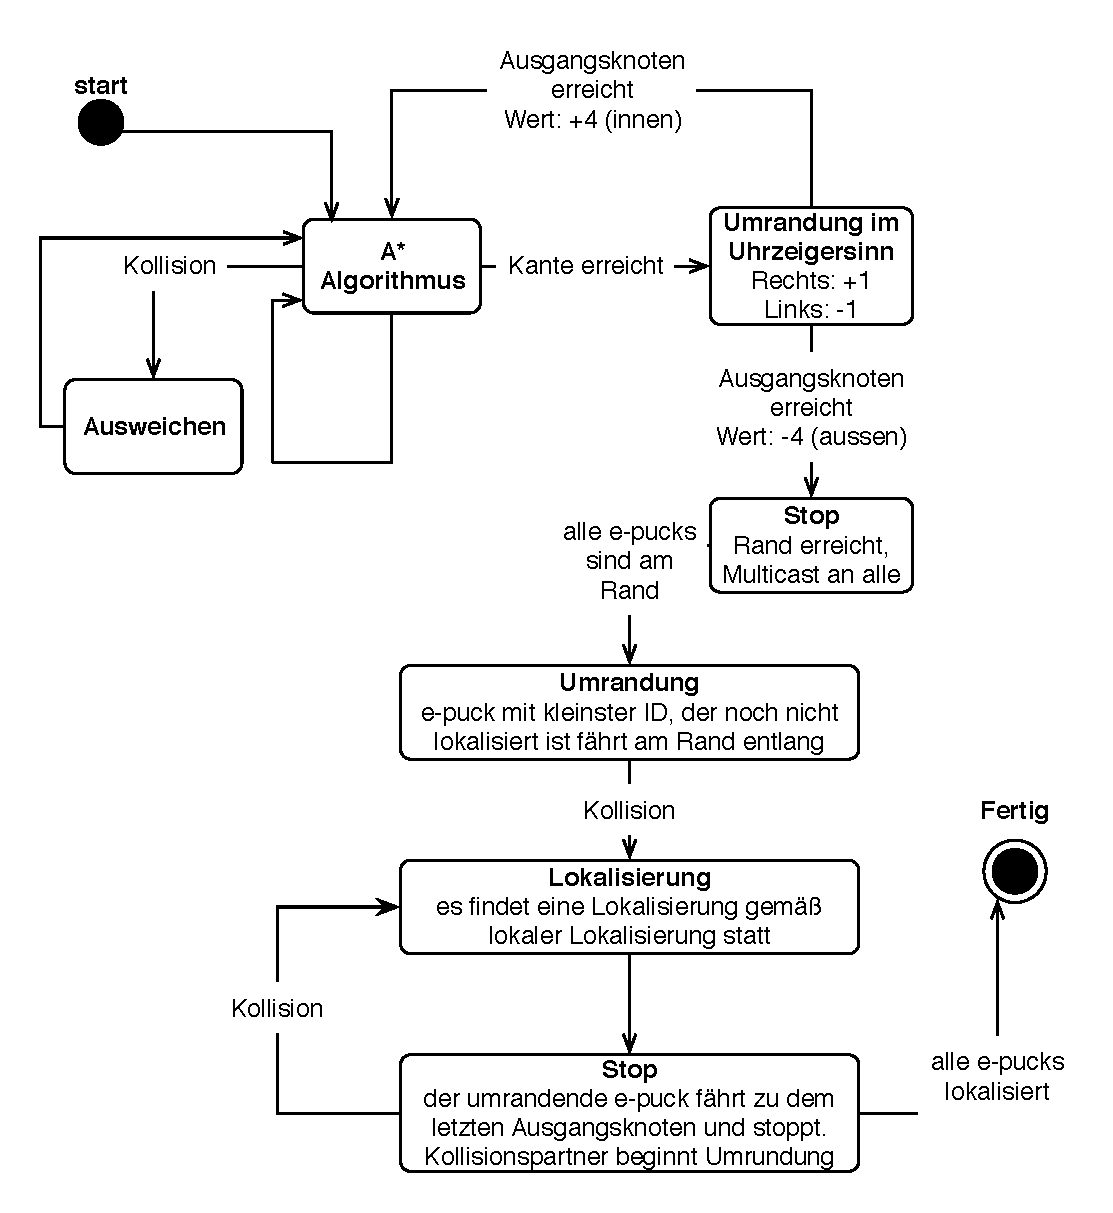
\includegraphics[width=10cm]{images/globale_lokalisierung.eps}
  				\caption{Zustandsdiagramm - Algorithmus zur globalen Lokalisierung}
  				\label{fig:globale_lokalisierung}
  			\end{figure}
  			Die Fahranweisungen erhält der Roboter über den A$^\ast$ Suchalgorithmus, somit fährt er stets zum nächsten (``günstigsten'') unbekannten
  			Knoten. Die Randerkennung geschieht durch die 'Rechte-Hand-Regel'. Sobald ein Roboter einen Randknoten erkannt hat, umrandet er im
			mit Hilfe der ``Rechten-Hand-Regel'' den Randbereich. Jede Linkskurve wird hierbei mit $+1$ gewertet, jede Rechtskurve mit $-1$. Erreicht der Roboter wieder
			den Anfangsknoten und ist die Summe $+4$, so weiß er, dass er sich auf einem äußeren Rand befindet. Ist die Summe allerdings $-4$
			so befindet er sich auf einem inneren Randstück. Die Suche muss in diesem Fall mit Hilfe des A$^\ast$ Suchalgorithmus fortgesetzt werden.	
	\section{Kommunikation}
		\subsection{Nachrichtenverarbeitung}
			{Abgesehen von der anfänglichen Initialisierung des Bluetooth-Moduls, verläuft die Übertragung in beide
			Richtungen transparent über den primären UART des e-pucks mit der {\tt hal\_uart1} Schicht. Jeder e-puck besitzt
			sowohl einen Eingangs- als auch	einen Ausgangsringpuffer über welche die Nachrichten von der Hardware empfangen
			bzw. gesendet werden. Die Logik des e-pucks verwendet lediglich die {\tt com}-Schicht um Nachrichten zu
			empfangen bzw. zu senden. Dazu wird der Eingangspuffer von der Logik überwacht. Sobald mindestens eine Nachricht
			vorhanden ist, wird diese über die	{\tt com}-Schicht ausgelesen und an den von der Logik festgelegten Callback
			übergeben.

			Jede e-puck Antwortnachricht hat eine vorhergehende Android-Anfragenachricht (siehe Abbildung \ref{fig:nachrichtensequenzen}) als Ursache.
		 	\begin{figure}[h]
				\centering
				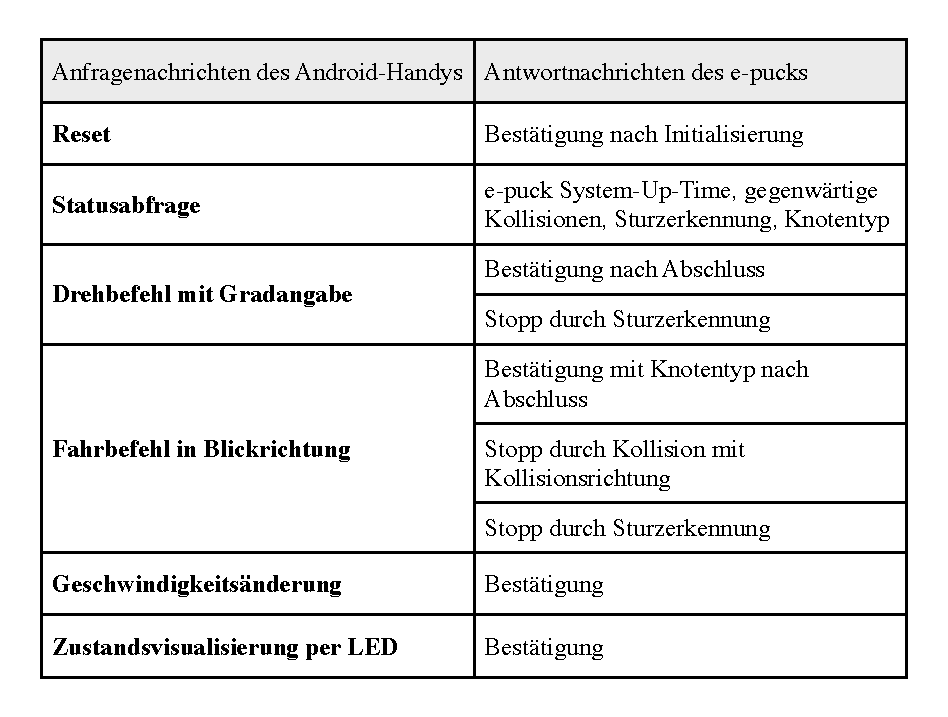
\includegraphics[width=10cm]{images/epuck_bt_msgs.eps}
  				\caption{Nachrichtensequenzen}
  				\label{fig:nachrichtensequenzen}
  			\end{figure}					
			}
		\subsection{Nachrichtenformat}
			\begin{itemize}
				\item Jede Nachricht besteht aus 32 Bytes
				\item Das Zahlenformat ist Little-Endian
				\item Die ersten beiden Bytes identifizieren den Nachrichtentyp eindeutig
				\item Die verbleibenden 30 Bytes können nachrichtenspezifisch verwendet werden
			\end{itemize}			
	\newpage	
	%Glossar ausgeben
	\printglossary[style=altlist,title=Glossar]
						
\end{document}
